% !TEX encoding = IsoLatin
\documentclass[12pt, a4paper, french]{article}
\usepackage[utf8]{inputenc}
\usepackage{lmodern}
\usepackage[T1]{fontenc}
%\usepackage[latin1]{inputenc}
\usepackage[hmargin = 25mm, vmargin = 25mm]{geometry}
%\geometry{letterpaper}                   % ... or a4paper or a5paper or ... 
%\geometry{landscape}                % Activate for for rotated page geometry
%\usepackage[parfill]{parskip}    % Activate to begin paragraphs with an empty line rather than an indent
\usepackage{graphicx}
\usepackage{amssymb, amsmath, amsthm}
\usepackage{epstopdf}
\usepackage{moreverb,stmaryrd}
\usepackage{natbib}
\usepackage[nottoc,notlot,notlof]{tocbibind}
\usepackage{hyperref}
\usepackage{algorithm,algorithmic}
\usepackage[french]{babel}
\usepackage{hyperref}
\usepackage{fancyhdr} 
\usepackage{booktabs}
\usepackage{longtable}
\usepackage{array}
\usepackage{multirow}
\usepackage[table]{xcolor}
\usepackage{wrapfig}
\usepackage{float}
\usepackage{colortbl}
\usepackage{pdflscape}
\usepackage{tabu}
\usepackage{threeparttable}
\usepackage{threeparttablex}
\usepackage[normalem]{ulem}
\usepackage{makecell}

\pagestyle{fancy}
\renewcommand{\headrulewidth}{0pt}
\fancyhead[C]{} 
\fancyhead[L]{}
\fancyhead[R]{}

\renewcommand{\footrulewidth}{0pt}
\fancyfoot[C]{\footnotesize{$13^{es}$ Journées de méthodologie statistique de l’Insee (JMS) / 12-14 juin 2018 / PARIS}}
\fancyfoot[R]{\thepage}

\begin{document}
\newcommand{\inter}[2]{\llbracket  #1\,,\, #2  \rrbracket}
\pagenumbering{roman}

\begin{center}

\includegraphics[width=15cm]{img/head_jms2018.png} 
\line(1,0){450}
\vspace{5mm}
\textbf{{\huge D}\Large U BON USAGE DES MOD\`ELES REG-ARIMA EN D\'ESAISONNALISATION}
\end{center}

\begin{center}
\textit{Alain QUARTIER-LA-TENTE(*), Dominique LADIRAY (*)} \\
%- N. B. le premier nom doit être celui de l'auteur qui effectuera la présentation orale (sauf contributions associées)
\vspace{2mm}
\textit{(*) INSEE, Département des Méthodes Statistiques}\\ 
\vspace{2mm}
\url{alain.quartier-la-tente@insee.fr} 
\end{center}
\vspace{5mm}
\small{{\bf Mots-cl\'es.} Désaisonnalisation, modèles Reg-ARIMA, effets de calendrier, points atypiques.}

\begin{center}
\line(1,0){450}
\end{center}


\section*{Résumé}
Les modèles de régression avec erreurs ARIMA (Reg-ARIMA) sont aujourd'hui largement utilisés en désaisonnalisation pour enlever des effets déterministes présents dans la série (points atypiques, ruptures, effets de calendrier) avant de la décomposer en tendance-cycle, saisonnalité et irrégulier.

Les principaux logiciels d’ajustement saisonnier (\textsc{X-13Arima-Seats}, \textsc{Tramo-Seats}, \textsc{JDemetra+}) mettent en œuvre ces modèles de façon automatique et très conviviale. Cette facilité cache en fait une complexité réelle et dans certains cas un manque de robustesse qui peut échapper à l’utilisateur.

Dans cette présentation, nous attirons l'attention sur les réelles difficultés de mise en œuvre de ces modèles à travers des cas concrets : l’estimation d’un effet d’année bissextile, l’estimation de ruptures et même l’estimation d’un modèle ARIMA.

\section*{Abstract}

Regression models with ARIMA errors (Reg-ARIMA) are nowadays commonly used in seasonal adjustment to remove the main deterministic effects (outliers, ruptures, calendar effects) from the raw data before decomposing the corrected series into trend-cycle, seasonality and irregular.

The main seasonal adjustment programs (\textsc{X-13Arima-Seats}, \textsc{Tramo-Seats}, \textsc{JDemetra+}) implement these models in an automatic and very user-friendly way. This facility hides in fact a real complexity and in certain cases a lack of robustness which can escape the user.

In this presentation, we draw attention to the real difficulties of implementing these models through concrete cases: the estimation of a leap year effect, the estimation of breaks and even the estimation of an ARIMA model.

\newpage

\tableofcontents

\newpage


\listoftables
\listoffigures

\newpage

\pagenumbering{arabic}
\section*{Introduction \markboth{Introduction}{Introduction}}
\addcontentsline{toc}{section}{Introduction} 

Les méthodes de désaisonnalisation les plus populaires sont sans nul doute \textsc{Tramo-Seats}, voir \cite{GM1996} et \cite{MC2004}, une méthode paramétrique basée sur les modèles ARIMA et \textsc{X-13Arima-Seats}, voir \cite{FMBOC1998} ou \cite{LQ2001}, une méthode non-paramétrique basée sur les moyennes mobiles.
Ces deux méthodes sont d'ailleurs recommandées par Eurostat et la Banque centrale européenne (BCE) pour la désaisonnalisation des indicateurs économiques.

Ces méthodes procèdent en deux étapes résumées dans la figure (\ref{fig:X13TS}). Dans un premier temps, elles corrigent la série à désaisonnaliser de certains effets déterministes (points atypiques, ruptures, effets de calendrier) et, dans un second temps elles décomposent la série ainsi «~nettoyée~» en tendance-cycle, composante saisonnière et composante irrégulière.

\begin{figure}[!ht]
\begin{center}
 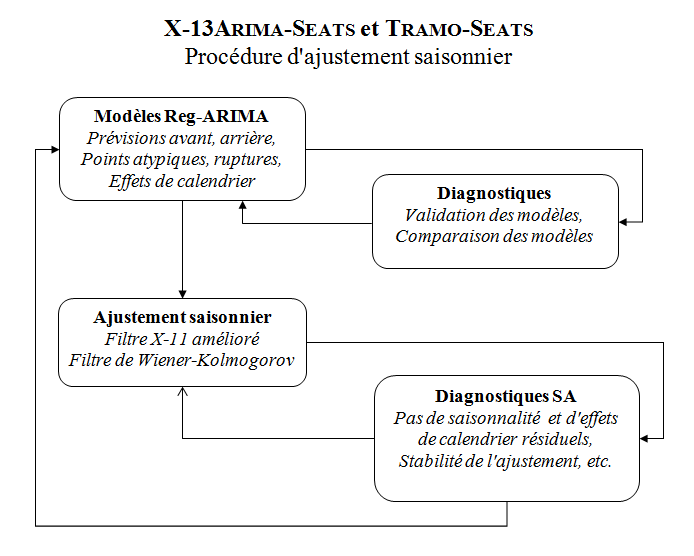
\includegraphics[scale=0.8]{img/MethodesX13-TS.png}
 \caption{Le fonctionnement global de \textsc{X-13Arima-Seats} et \textsc{Tramo-Seats} : correction et décomposition.}
 \label{fig:X13TS}
\end{center}
\end{figure}

L'étape préalable à la décomposition, dite de pré-ajustement, repose sur un modèle de «~régression avec erreurs ARIMA~» (modèle Reg-ARIMA). Un algorithme de modélisation automatique (AMI) est à la disposition de l'utilisateur qui permet:
\begin{itemize}
  \item[$\bullet$] de déterminer le modèle de composition de la série (additif ou multiplicatif) ;
	\item[$\bullet$] de détecter et corriger les ruptures dans la série ; 
	\item[$\bullet$] de détecter et corriger les éventuels effets de calendrier (effets de jours ouvrables et effets de fêtes mobiles comme Pâques) ;
	\item[$\bullet$] d'ajuster aux «~résidus~» de la régression un modèle ARIMA ;
	\item[$\bullet$] d'estimer les éventuelles valeurs manquantes ;
	\item[$\bullet$] et enfin de prévoir et de rétropoler la série étudiée.
\end{itemize}

Cet algorithme automatique est mis en œuvre de façon très conviviale dans les logiciels et est toujours accompagné d'une large batterie de tests statistiques permettant de juger de la qualité de l'ajustement fait. On en trouvera une description très détaillée dans \cite{GM1998}.

\cite{MLP2015}, \cite{MLP2016}, \cite{M2018} évaluent les performances de cet AMI. Leurs résultats sont élogieux pour cet outil mais ils considèrent d'une part une modélisation à un instant donné et ils valident d'autre part la méthode par les tests qui ont finalement servis à la bâtir. Il n'en reste pas moins que l'AMI est un outil \textbf{exploratoire} de premier ordre, malheureusement trop souvent utilisé en pratique comme une boîte noire.

\vskip \baselineskip
L'objectif de cette présentation est, à partir de simulations simples sur données réelles et en se concentrant sur la stabilité des estimations, de montrer que ces modèles Reg-ARIMA sont complexes, difficiles à utiliser, et qu'il faut les manier avec prudence.

Dans une première partie, nous rappelons brièvement la définition des modèles Reg-ARIMA et les principales composantes déterministes retenues dans ce travail. La seconde partie de l'étude est consacrée à l'estimation d'un effet d'année bissextile dans les séries de l'indice de la production industrielle (IPI) et de l'indice de chiffre d'affaires (ICA) de pays de l'union européenne. La troisième partie se consacre à l'estimation de 4 types de ruptures --- les points atypiques, les changements transitoires de niveau, les changements de niveau et les ruptures saisonnières --- dans les séries de l'IPI. La quatrième partie s'intéresse à l'estimation même du modèle ARIMA.

Cette présentation ne \textbf{démontre} rien : elle se contente de \textbf{montrer} sur des exemples concrets, que la modélisation Reg-ARIMA souffre, comme nombre de méthodes paramétriques, d'un certain manque de robustesse. L'utilisation de ces modèles, par ailleurs très performants, demande à la fois une bonne connaissance de la théorie sous-jacente et de ses limites, et une grande prudence comme le résument bien \cite{FMcE2018} :
\begin{quote}
«~\textit{ARIMA Model-Based Seasonal Adjustment (AMBSA) should not be a black box procedure to its users because default software procedures are sometimes seriously inadequate. Also user decisions regarding software options and model choice can strongly impact the results obtained, for better or worse. A seasonal adjuster who understands the basic facets of the method and some of its diagnostics, as outlined and then detailed in this document, will have a greater capacity to obtain successful adjustments}~».
\end{quote}

\vskip \baselineskip


\section{Les modèles Reg-ARIMA}

\subsection{Définition}

Soit $z_t$ une série observée, mensuelle ($s=12$) ou trimestrielle ($s=4$) et le cas échéant transformée par logarithme. \textsc{X-13Arima-Seats} et \textsc{Tramo-Seats} ajustent à $z_t$ un modèle du type :
\begin{equation}
 \begin{array}{lcl}
   z_t & = & y'_t\beta + x_t \\
	\phi(B)x_t & = & \Theta(B)  a_t,
 \end{array}
 \label{eq:eq1}
\end{equation}
où :
\begin{itemize}
	\item[$\bullet$] $y'_t\beta$ est le terme de régression prenant en compte les composantes déterministes de la série, dont le terme constant,
	\item[$\bullet$] $x_t$, le «~résidu~», suit un modèle ARIMA $(p,d,q)(P,D,Q)_s$,
	\item[$\bullet$] $\phi(B)$ et $\Theta(B)$ sont des polynômes de l'opérateur retard $B$ ($B^j  z_t=z_{t-j}$),
	\item[$\bullet$] et $a_t$ est un bruit blanc.
\end{itemize}
\vskip \baselineskip
Pour des séries saisonnières, une spécification multiplicative est retenue :
\begin{equation}
	\varphi_r (B) \varphi_s (B^s ) \nabla^D \nabla_s^{D_s}   x_t = \theta_r (B) \theta_s (B^s)  a_t,
	\label{eq:eq2}
\end{equation}
où :
\begin{itemize}
	\item[$\bullet$] ($\nabla^D, \nabla_s^{D_s}$) est la différenciation qui conduit à la stationnarité, avec $\nabla^D = (1-B)^D$ et $\nabla^{D_s}_s=(1-B^s)^{D_s}$,
	\item[$\bullet$] $\varphi_r (B)$  et $\varphi_s (B^s)$ sont les polynômes autoregressifs associés aux parties stationnaires régulière et saisonnière, d'ordre $P_r$ and $P_s$ : 
$$
\begin{array}{lcl}
\varphi_r (B)   & = & 1 + \varphi_{r,1} (B) + \cdots + \varphi_{r,P_r} (B^{P_r}) \\
\varphi_s (B^s) & = & 1 + \varphi_{s,1} (B^s) + \cdots + \varphi_{s,P_s} (B^{sP_s}),
\end{array}
$$
	\item[$\bullet$] $\theta_r (B)$  et $\theta_s (B^s)$ sont les polynômes moyennes mobiles associés aux parties régulière et saisonnière, d'ordre $Q_r$ et $Q_s$ : 
$$
\begin{array}{lcl}
\theta_r (B)   & = & 1 + \theta_{r,1} (B) + \cdots + \theta_{r,Q_r} (B^{Q_r}) \\
\theta_s (B^s) & = & 1 + \theta_{s,1} (B^s) + \cdots + \theta_{s,Q_s} (B^{sQ_s}),
\end{array}
$$
	\item[$\bullet$] et $a_t$ est un bruit blanc.
\end{itemize}

Dans l'algorithme automatique mis en œuvre par \textsc{X-13Arima-Seats} et \textsc{Tramo-Seats}, l'ordre des polynômes est contraint : $P_r\text{ et }Q_r\in \inter{0}{3}$, $D\in \inter{0}{2}$ et $D_s,\, P_s \text{ et } Q_s\in \inter{0}{1}$, ce qui correspond à 384 modèles ARIMA possibles. 

% $0 \leq P_r$ et  $Q_r \leq 3$, $0 \leq D \leq 2$, $0 \leq D_s \leq 1$, $0 \leq P_s$ et $Q_s \leq 1$, ce qui correspond à 384 modèles ARIMA possibles.

\subsection{Les composantes déterministes de la régression.}

En désaisonnalisation, on se concentre traditionnellement sur deux composantes importantes : les effets de calendrier, qu'il faut éliminer dans la série dite «~désaisonnalisée et corrigée des effets de jours ouvrables~» (CVS-CJO) et la présence de ruptures qui peuvent gêner par la suite l'estimation de la composante saisonnière.

\subsubsection{Les effets de calendrier.}

Les différents effets de calendriers, les modèles associés et les problèmes liés à leur détection et à leur estimation sont présentés en détail dans \cite{L2018}. Nous nous concentrons ici sur les effets dits de «~jours ouvrables~» liés au fait que la composition en jours des mois --- les nombres de lundis, mardis, \dots, dimanche --- varie au cours du temps.

En suivant les notations de \cite{FMBOC1998}, on suppose que le $j^{\mbox{\tiny {\`{e}me}}}$ jour de la semaine a un effet $\alpha_j$ où, par exemple, $j=1$ désigne le lundi, $j=2$ le mardi, \dots, et $j=7$ le dimanche. Chaque $\alpha_j$ représente par exemple les ventes moyennes d'un jour $j$. Si $N_{jt}$ représente le nombre de jours $j$ dans le mois $t$, la longueur du mois $t$ est alors $N_t = \sum_{j=1}^{j=7} N_{jt}$ et l'effet cumulé pour ce mois (les ventes totales du mois) sera :
$TD_t = \sum_{j=1}^{j=7} \alpha_j N_{jt}$.

Une première idée pour détecter et évaluer les effets de jours ouvrables dans une série est d'expliquer les valeurs de la série par les 7 variables $N_{jt}$. Mais ces régresseurs sont par nature saisonniers (il y a en moyenne plus de lundis en janvier qu'en février) et fortement corrélés. 

Une formulation différente mais équivalente de l'effet jours ouvrables permet de résoudre en grande partie ces problèmes. L'effet journalier moyen, les ventes moyennes d'une journée, s'écrit $\bar{\alpha} = \sum_{j=1}^7 \alpha_j /7$. 
Comme par construction $\sum_{j=1}^7 \left(\alpha_j-\bar{\alpha}\right) = 0$, on peut écrire :
\begin{eqnarray*}
\sum_{j=1}^7 \alpha_j N_{jt} & = & \bar{\alpha}N_t + \sum_{j=1}^7 \left(\alpha_j-\bar{\alpha}\right) N_{jt} \nonumber \\
& = &  \bar{\alpha}N_t + \sum_{j=1}^6 \left(\alpha_j-\bar{\alpha}\right) \left(N_{jt} - N_{7t}\right).
\end{eqnarray*}
Ainsi, l'effet cumulatif du mois se décompose en un effet directement lié à la longueur du mois et un effet net de chaque jour de la semaine. Comme la quantité $\bar{\alpha}N_t$ est par nature saisonnière (janvier a toujours plus de jours que février), on utilise en fait l'égalité : $\bar{\alpha}N_t = \bar{\alpha}N_t^* + \bar{\alpha}\left(N_t-N_t^*\right)$, où $N_t^*$
représente la moyenne de la longueur du mois $t$. En d'autres termes, $N_t^*$  est égal à $30$ ou $31$ si le mois considéré n'est pas un mois de février et à $28,25$\footnote{En fait, la vraie valeur serait $28,2425$ comme indiqué dans l'annexe (\ref{sec:cal}).} dans le cas contraire. Le second terme de l'égalité est donc nul sauf pour le mois de février. L'utilisation des variables contrastes permet donc de désaisonnaliser les régresseurs jours ouvrables.

Les versions actuelles de \textsc{X-13Arima-Seats} et \textsc{Tramo-Seats} utilisent le modèle Reg-ARIMA suivant pour estimer les effets de jours ouvrables :
\begin{eqnarray}
	\label{eq:eq3}
z_t=\beta_0 LY_t + \sum_{j=1}^{j=6} \beta_j \left(N_{jt} - N_{7t}\right) + x_t,
\end{eqnarray}
où $LY_t$ désigne le régresseur «~année bissextile~» --- \emph{Leap Year} (LY) --- égal à:
\[
LY_{t} = \left\{ \begin{array}{rl} 
                0,75 & \mbox{si } t \mbox{ est un mois de février bissextil } \\
                -0,25 & \mbox{si } t \mbox{ est un mois de février non bissextil } \\
                0 & \mbox{sinon}
               \end{array}
         \right.
\]


\subsubsection{Points atypiques et ruptures.}
\label{sec:PAR}

Les différents types de rupture, les modèles associés et les problèmes liés à leur détection et à leur estimation sont présentés en détail dans \cite{Me2018}.

Dans la suite, nous nous intéresserons aux ruptures suivantes :
\begin{itemize}
	\item[$\bullet$] Le point atypique $AO$ («~\emph{additive outlier}~») qui représente une rupture dans la série n'affectant qu'une observation, un mois. Les $AO$ sont modélisés par des régresseurs du type : 
	
$
AO_{t} = \left\{ \begin{array}{cl} 
                1 & \mbox{si } t=t_{0} \\
                0 & \mbox{si } t\neq t_{0}
               \end{array}
       \right.
$
	\item[$\bullet$] Le changement de niveau $LS$ («~\emph{level shift}~») qui représente une rupture permanente dans le niveau de la série. Les $LS$ sont modélisés par des régresseurs du type : 
	
$
LS_{t} = \left\{ \begin{array}{rl} 
                -1 & \mbox{si } t<t_{0} \\
                0 & \mbox{si } t\geq t_{0}
               \end{array}
       \right.
$
	\item[$\bullet$] Le changement transitoire de niveau $TC$ («~\emph{transitory change}~») qui représente une rupture dans la série suivie d'un retour progressif à la normale. Les $TC$ sont modélisés par des régresseurs du type : 
	
$
TC_{t} = \left\{ \begin{array}{cl} 
                0 & \mbox{si } t<t_{0} \\
                \alpha^{t-t_{0}} & \mbox{si } t \geq t_{0}
               \end{array}
       \right.
$

où $\alpha$, qui traduit la vitesse de retour à la normale, est pris par défaut égal à 0,7.
	\item[$\bullet$] La rupture dans la composante saisonnière $SO$ («~\emph{seasonal outlier}~») qui traduit une rupture permanente dans le coefficient saisonnier d'un mois. Les $SO$ sont modélisés par des régresseurs du type : 
	
$			
SO_{t} = \left\{ \begin{array}{cl} 
                0 & \mbox{si } t \geq t_{0} \\
								1 & \mbox{si } t < t_{0} \mbox{ et } t  \mbox{ même mois/trimestre que } t_{0}\\
                -1/(s-1) & \mbox{sinon }
               \end{array}
       \right.		
$
\end{itemize}

\vskip \baselineskip

La figure (\ref{fig:Outliers}) donne une représentation graphique des régresseurs associés à ces 4 types de rupture.

Les AO et LS sont relativement fréquents dans les séries économiques. Les SO et TC beaucoup plus rares et souvent difficiles à expliquer du point de vue économique. D'autres types de ruptures sont parfois considérés: les rampes $RP$ (changement progressif de niveau), les changements temporaires de niveau $TLS$, etc.


\begin{figure}[!ht]
\begin{center}
 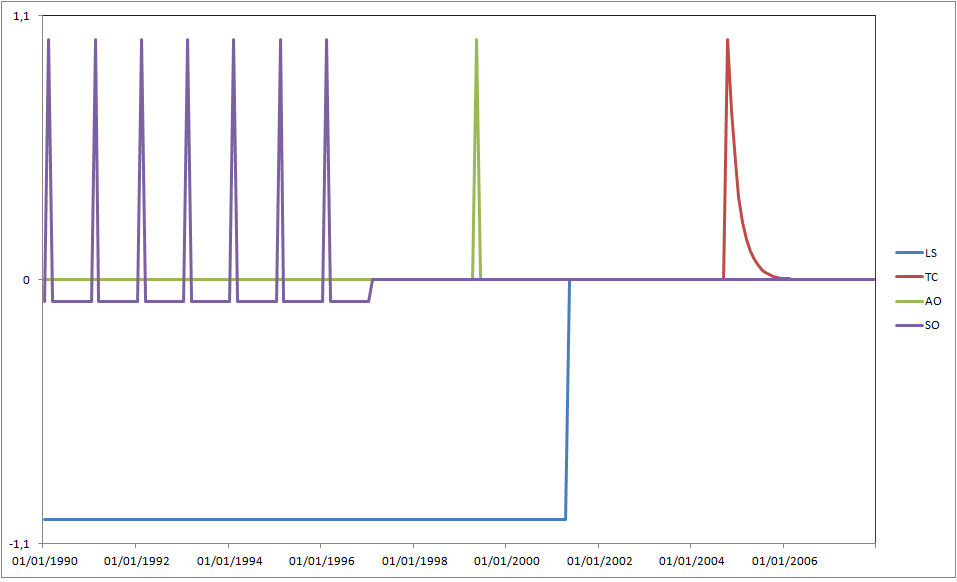
\includegraphics[scale=0.65]{img/Outliers.png}
 \caption{Régresseurs associés à certaines formes de rupture (AO, LS, TC, SO).}
 \label{fig:Outliers}
\end{center}
\end{figure}


\subsection{Un exemple avec \textsc{X-13Arima-Seats}}

À titre d'exemple, la figure (\ref{fig:IPI}) montre le résultat du traitement automatique de l'IPI de l'industrie manufacturière en France (NAF révision 2, niveau A10, poste CZ), de janvier 2006 à avril 2017. Les calculs ont été faits avec le logiciel \textsc{JDemetra+}\footnote{JDemetra+ est le logiciel Européen recommandé par la BCE et Eurostat pour la désaisonnalisation des indicateurs économiques. Il met en œuvre en particulier les méthodes \textsc{X-13Arima-Seats} et \textsc{Tramo-Seats}.} version 2.2.1, en utilisant le module Reg-ARIMA mis en œuvre dans \textsc{X-13Arima-Seats} et le système d'options par défaut «~RSA5c~», voir \cite{G2017} pour plus d'information.

Tous les indicateurs statistiques associés à ce calcul sont «~au vert~» (i.e. : considérés comme «~bons~» par JDemetra+) et le modèle final montre :
\begin{itemize}
	\item[$\bullet$] Un fort effet jours ouvrables avec un coefficient négatif attendu du weekend ;
	\item[$\bullet$] Un effet d'année bissextile attendu ;
	\item[$\bullet$] Un effet de Pâques plus surprenant ;
	\item[$\bullet$] Un point atypique en mai 2011 où la production semble avoir été beaucoup plus forte qu'attendue.
\end{itemize}
Débarrassée de ces effets déterministes, la série suit alors un modèle Airline $(0,1,1)(0,1,1)$.

\vskip \baselineskip

Ce simple exemple met en évidence certaines limites d'une utilisation «~aveugle~» de l'AMI : Pourquoi la production industrielle baisserait-elle la semaine précédant Pâques ? L'utilisation de l'option «~RSA5c~» revient à spécifier un type de modèle Reg-ARIMA et en particulier à envisager que l'IPI est influencé par la fête de Pâques. Si cette hypothèse pourrait être éventuellement acceptée pour certains secteurs (viande d'agneau, production de chocolat), elle semble farfelue au niveau global. Par contre, certains secteurs du commerce de détail pourraient eux présenter un effet Pâques (vente de chocolat, agneau, fleurs).

L'AMI, qui met en œuvre automatiquement la méthode de Box et Jenkins, aide l'analyste à formuler, \textbf{à spécifier}, un modèle en lui révélant l'éventuelle présence de points atypiques et de ruptures, d'effets de calendrier et en proposant un modèle ARIMA pour les résidus de ce modèle. Cet algorithme est particulièrement utile pour démarrer une analyse, surtout quand on a à traiter plusieurs dizaines ou centaines de séries. Il est aussi parfois utilisé dans une campagne annuelle de désaisonnalisation pour vérifier si d'autres modèles ne pourraient pas être substitués à ceux utilisés en production.

Il faut bien comprendre et garder en tête que cet outil est exploratoire. Malgré son exceptionnelle efficacité, ce n'est pas un outil confirmatoire et ses résultats n'ont aucun caractère de vérité absolue. Il est facile de le montrer:
\begin{itemize}
	\item[$\bullet$] Dans la pratique, il arrive souvent que le modèle proposé par l'AMI soit modifié : on pourra alors inclure en dur des points atypiques ou des ruptures, changer le système de régresseurs pour jours ouvrables, voire modifier le modèle ARIMA, etc.
	\item[$\bullet$] Il n'est pas rare que \textsc{Seats} rejette le modèle ARIMA proposé par \textsc{Tramo} pour choisir \emph{in fine} un modèle décomposable.
	\item[$\bullet$] Les algorithmes AMI de \textsc{X13-Arima-Seats} et \textsc{Tramo-Seats} sont différents et donnent des résultats différents. À titre d'illustration, les deux algorithmes ont été appliqués sur 205 séries de l'IPI: le modèle ARIMA n'est le même que dans 60~\% des cas et le diagnostic sur la significativité du jeu de régresseurs pour jours ouvrables est différent pour 10~\% des séries (voir tableau [\ref{table:CompareTSX13}]).
	\item[$\bullet$] Ces algorithmes utilisent de nombreux tests statistiques et sont très sensibles aux valeurs seuil préprogrammées. Ainsi, changer la valeur par défaut du test de significativité des points atypiques peut avoir des conséquences très importantes sur le modèle finalement proposé.
\end{itemize}

\begin{table}
\caption[Comparaison des résultats du model AMI de Tramo-Seats et X13 sur les 205 séries de l'IPI (cas TD6+LY)]{Comparaison des résultats du model AMI de Tramo-Seats et X13 sur les 205 séries de l'IPI (cas TD6+LY).}\label{table:CompareTSX13}
\begin{center}
\small
\begin{tabular}{lrr} \\
\hline
\rule{0pt}{3ex}Résultat&Model&Diagnostic sur JO ?  \\
\hline
Différent&  84&  22 \\
Identique& 121& 183 \\
\hline
Total& 205 & 205  \\
\hline
\end{tabular}
\normalsize
\end{center}
\end{table}

Nous allons illustrer dans la suite certains problèmes liés à une «~utilisation aveugle~» de cet algorithme en nous concentrant sur la stabilité et la pertinence des estimations du modèle Reg-ARIMA.

\begin{figure}[!ht]
\begin{center}
 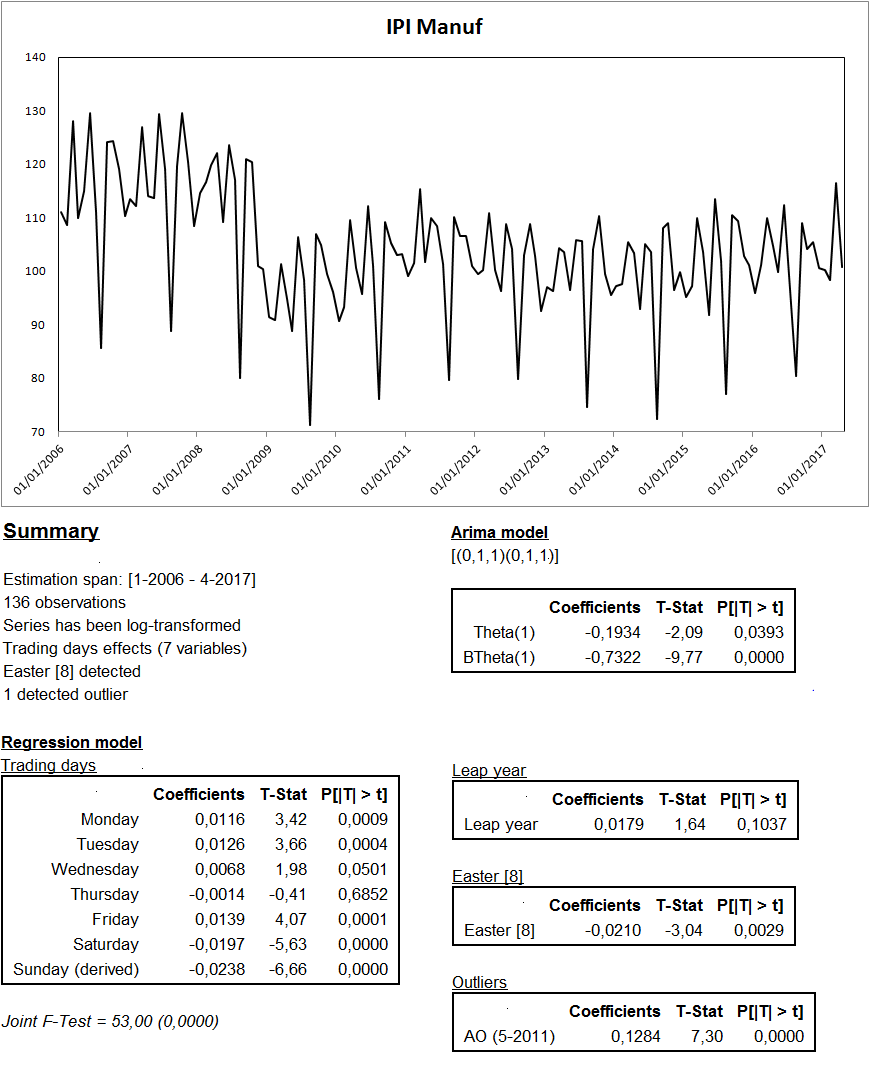
\includegraphics[scale=0.7]{img/IPImanuf.png}
 \caption[Modélisation automatique de l'IPI de l'industrie manufacturière en France]{Modélisation automatique de l'IPI de l'industrie manufacturière en France.}
 \label{fig:IPI}
\end{center}
\end{figure}

\clearpage

\section{Estimation d'un effet «~année bissextile~»}
\label{sec:LY}

Comme le montre l'équation (\ref{eq:eq3}), l'effet année bissextile est une composante à part entière de l'effet jours ouvrables généré par la composition en jours du mois variable d'une année et d'un mois à l'autre.

La présence de régresseurs pour jours ouvrables dans le modèle Reg-ARIMA implique d'une part que ces effets existent, d'autre part qu'ils sont en large partie indépendants du modèle ARIMA \footnote{C'est pour assurer au maximum cette indépendance que les régresseurs sont désaisonnalisés (c'est l'un des avantages de considérer des contrastes).}, et enfin qu'ils sont constants dans le temps.

Hormis l'hypothèse d'indépendance, ces points ne peuvent être validés qu'en considérant les séries traitées et en les replongeant dans leur contexte réel. Les lignes directrices sur la désaisonnalisation, \cite{E2015}, précisent d'ailleurs :

{\it «~The calendar adjustment should be done for those time series for which there is an economic rationale for the existence of calendar effects and statistical evidence.~»}

On suppose dans l'étude qui suit que la production industrielle et les chiffres d'affaires sont impactés par des effets de calendriers. C’est vrai sans aucun doute car ces effets résultent de diverses lois ou d'accords de branches : repos hebdomadaire obligatoire, en général le dimanche, jours fériés légaux, etc. Mais d'une part, il existe de nombreux aménagements possibles et d'autre part, les industries par exemple adaptent leur processus de production pour le rendre moins sensible aux congés, weekends, jours fériés, etc. Dans la pratique, on vérifie d'ailleurs aisément que le weekend est une période de production industrielle basse et que le samedi est un jour très favorable au chiffre d'affaires des commerces de détail.

De même, il est évident qu'il y a un effet d'année bissextile dans toutes les séries qui mesurent une activité mensuelle somme d'activités journalières\footnote{Il est cependant possible que cette «~évidence~» économique soit perturbée par la collecte statistique elle-même. Ainsi, dans le cadre de l'IPI certaines productions sont, ou ont été, mesurées en unités entières de production. Dans le cas de la fabrication d'avions ou de paquebots il est certain que l'effet année bissextile ne serait alors pas discernable du fait d'un biais lié à la troncature de la mesure au niveau mensuel. Ce type de problème est cependant moins courant dans la mesure où on compte de plus en plus les heures travaillées ou facturées.}. Une journée de plus ne peut qu'augmenter la production ou le chiffre d'affaires, et ce quoiqu'en disent le modèle Reg-ARIMA et les tests associés : en moyenne, cette augmentation sera de $(29/28 - 1) = 0,0357$ soit environ 3,6~\%. \cite{B1992} justifie ce chiffre pour un modèle multiplicatif et propose même dans ce cas de faire un ajustement préalable pour l'effet d'année bissextile plutôt que de l'estimer dans un modèle Reg-ARIMA, ce qui a donné naissance à l'option \emph{autoadjust} de \textsc{X13-Arima-Seats}.

\subsection{Méthodologie}

Dans cette étude sur la qualité de l'estimation de l'effet LY, nous utilisons les indices mensuels en volume de la production industrielle et de chiffre d'affaires des pays de la communauté européenne, aux niveaux 2, 3 ou quatre chiffres de la NACE rev 2. Nous conservons, pour étudier la convergence des estimations, les séries de plus de 12 ans. Au total, 2198 séries participent à la simulation\footnote{Ces séries sont disponibles sur le site d'Eurostat, dans les tables \emph{sts\_intv\_m}, \emph{sts\_setu\_m}, \emph{sts\_sepr\_m} et \emph{sts\_inpr\_m}. \url{http://ec.europa.eu/eurostat/data/database}.}.

Pour chaque série, nous procédons ainsi :
\begin{enumerate}
	\item Dans un premier temps, le modèle de décomposition, les points atypiques, les ruptures, les effets de jours ouvrables et le modèle ARIMA sont déterminés sur l'ensemble de la série. Le modèle Reg-ARIMA est donc déterminé.
	\item Dans un second temps, le modèle Reg-ARIMA est ré-estimé sur les 48 premières observations de la série, pour être certain d'observer au moins une année bissextile.
	\item Enfin, le processus est répété en ajoutant à chaque fois une observation, ce qui donne de nouvelles estimations des paramètres. Pour une série de 13 ans, nous aurons donc $12\times13 - 48 = 108$ estimations du coefficient de la variable LY.
\end{enumerate}
Ces simulations permettent alors d'étudier la convergence du coefficient LY. Dans cette étude, nous dirons que l'estimation du coefficient LY aura convergé lorsqu'elle restera à la fois positive, statistiquement significative et non significativement différente de la dernière estimation.

D'autres spécifications sont bien entendu possibles pour cette simulation : raccourcir la période d'estimation initiale, ne pas fixer le modèle, etc. Nous avons procédé à différentes expériences qui conduisent à des résultats similaires. Seuls les résultats de cette simulation à modèle Reg-ARIMA fixé sont présentés ici.

\subsection{Résultats}

Dans l'estimation de cet effet LY, un modèle Reg-ARIMA se retrouve naturellement confronté à plusieurs difficultés :
\begin{itemize}
	\item[$\bullet$] Tout d'abord, le manque de données : pour identifier l'effet d'une année bissextile, encore faut-il observer des années bissextiles \dots et suffisamment.
	\item[$\bullet$] La difficulté d'isoler chaque composante, on rappelle qu'elles ne sont pas observées directement, en particulier lorsque la série est très bruitée.
\end{itemize}

Les principaux résultats sont finalement assez bien résumés dans les graphiques (\ref{fig:LYexemple1}) et (\ref{fig:LYexemple2}) ; dans ces graphiques, les zones grisées représentent les intervalles de confiance à 90~\% et 95~\%.
\begin{itemize}
	\item[$\bullet$] Dans les deux cas, on voit que le coefficient LY met du temps à converger et les valeurs des premières années sont particulièrement erratiques.
	\item[$\bullet$] La première année bissextile est observée ici en 1992, et les autres en 1996, 2000, 2004, etc. Ce n'est qu'à partir de 2004 que le coefficient converge pour la série RF0610 ; la convergence est beaucoup plus lente pour la série RF1391.
	\item[$\bullet$] Les valeurs estimées pour la série RF1391 ne sont pas justifiables économiquement : comment un jour de plus dans un mois pourrait-il augmenter la production, toutes choses égales par ailleurs, de 7~\% à 14~\%, voire même 19~\% ?
\end{itemize}


\begin{figure}[!ht]
\begin{center}
 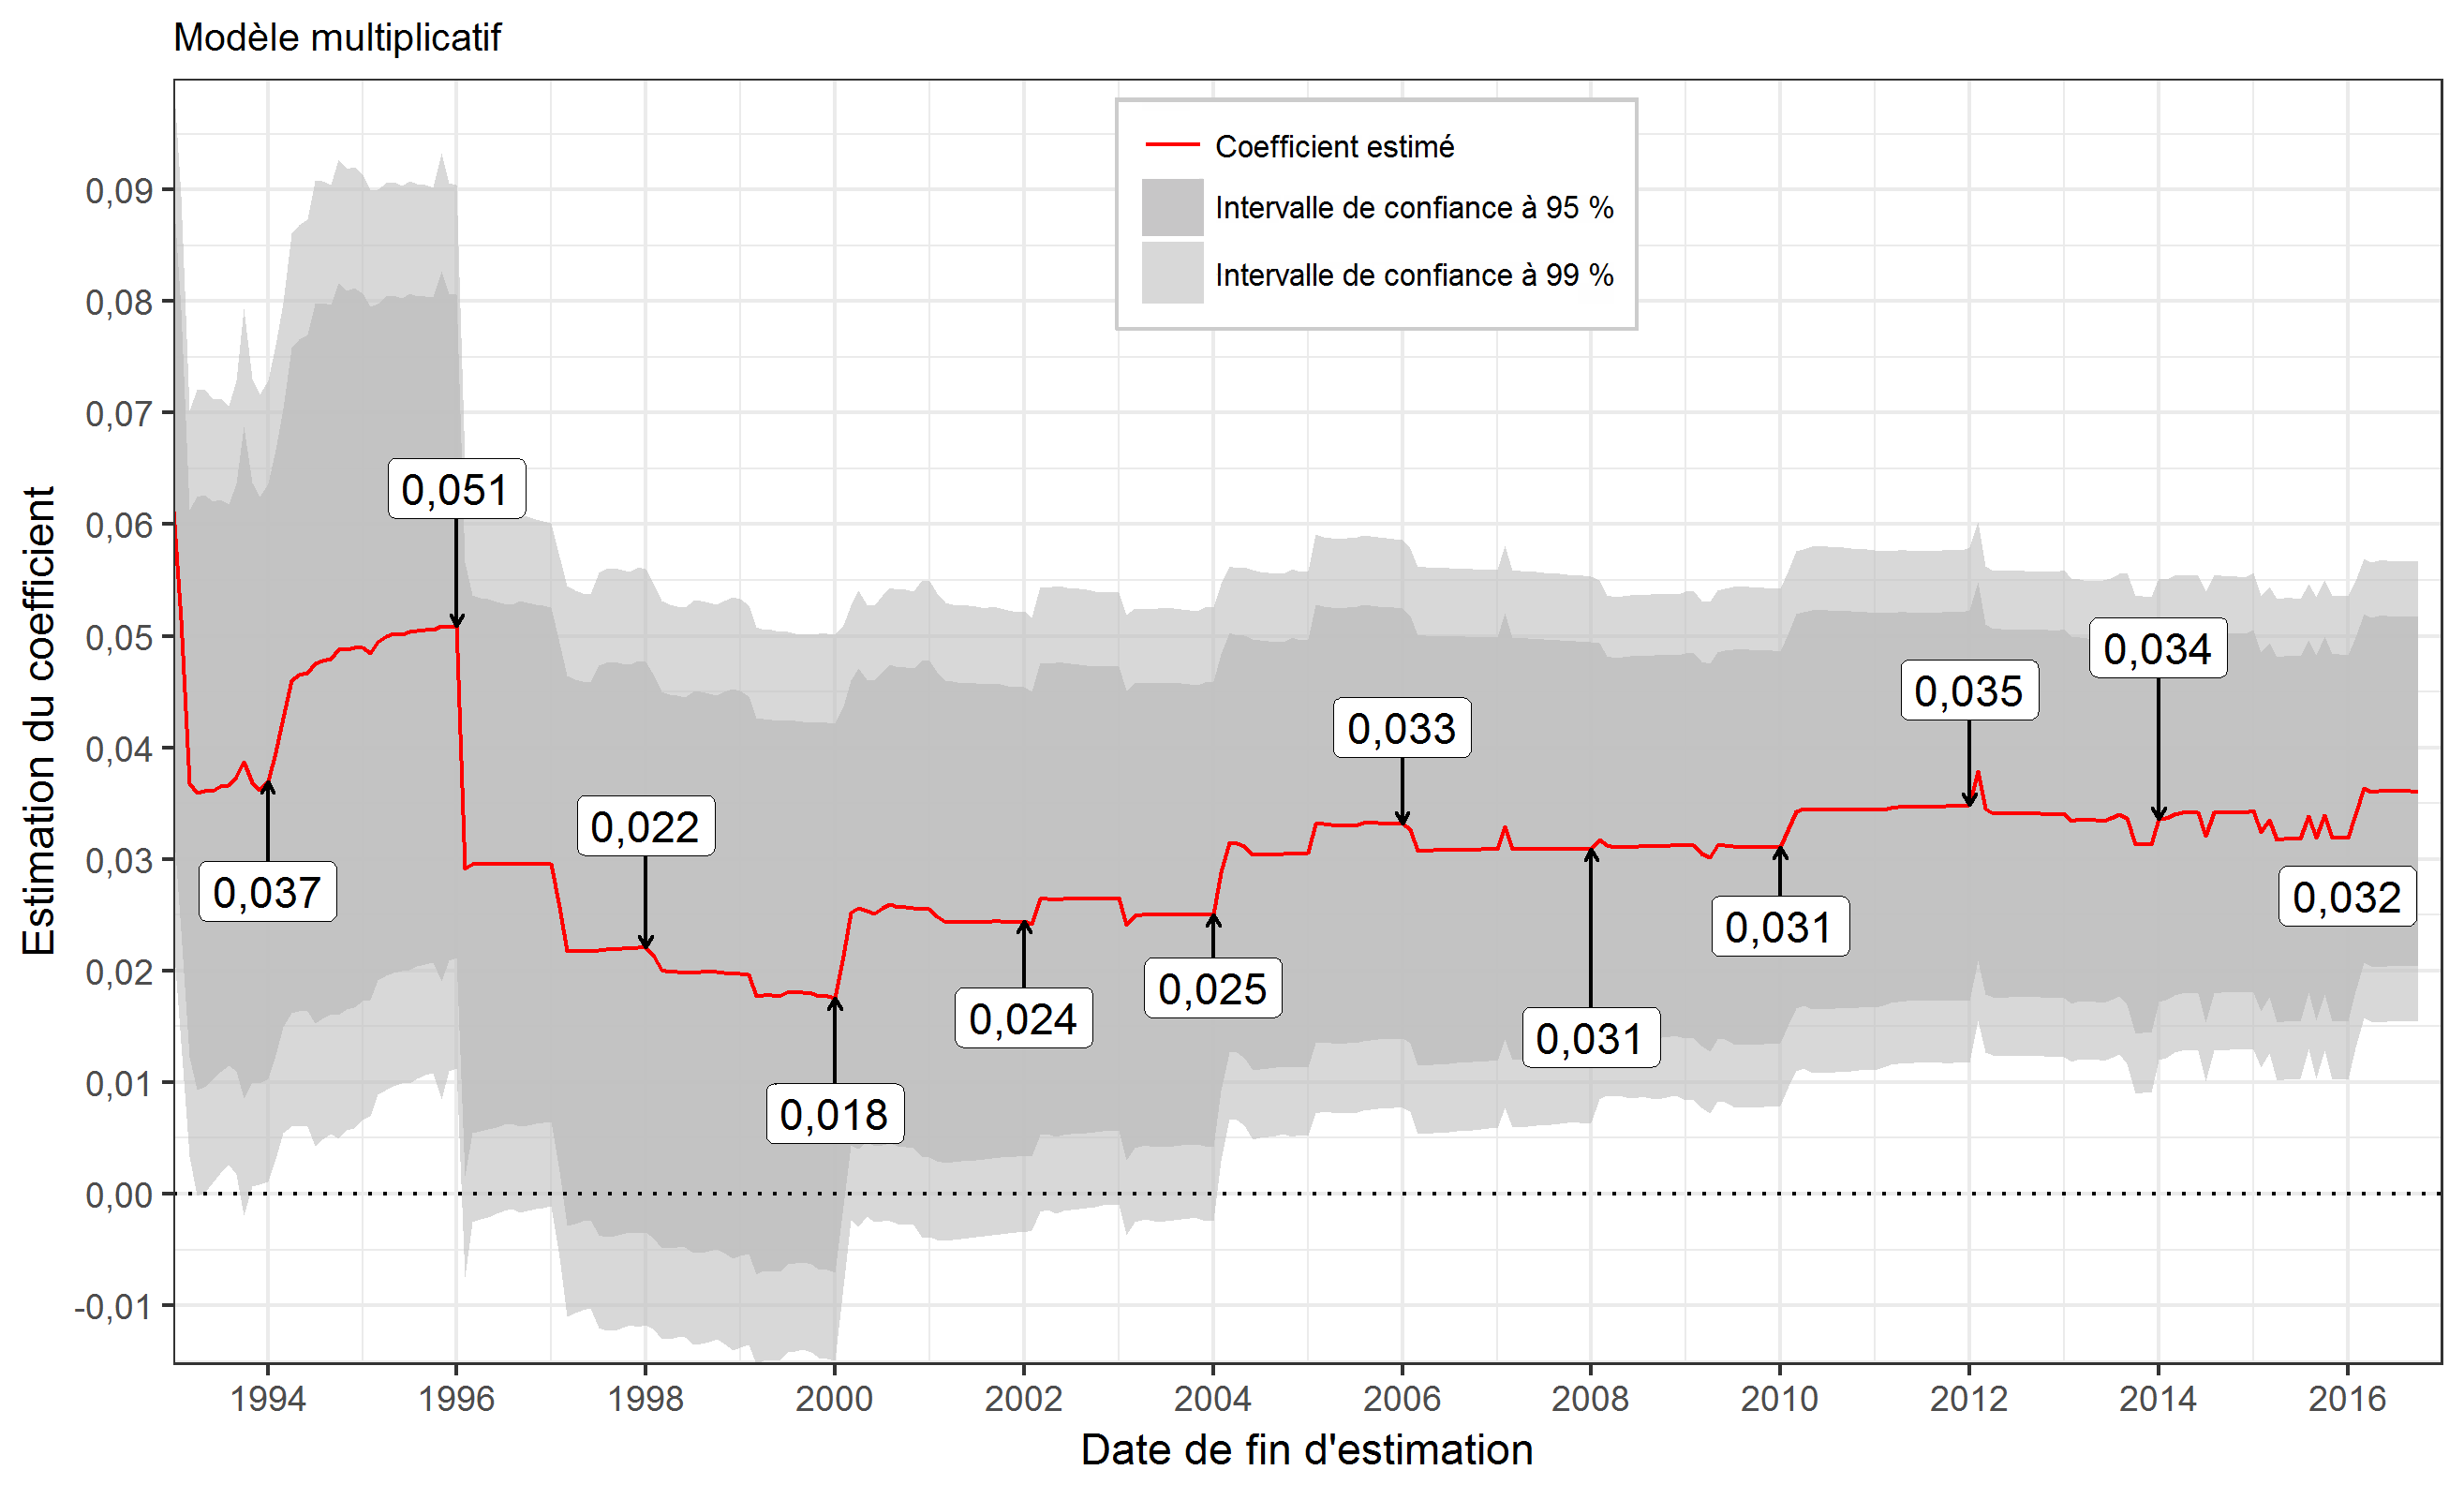
\includegraphics[scale=0.50]{img/LYexemple1.png}
 \caption{Estimations successives du coefficient LY pour la série RF0610.}
 \label{fig:LYexemple1}
\end{center}
\end{figure}

\begin{figure}[!ht]
\begin{center}
 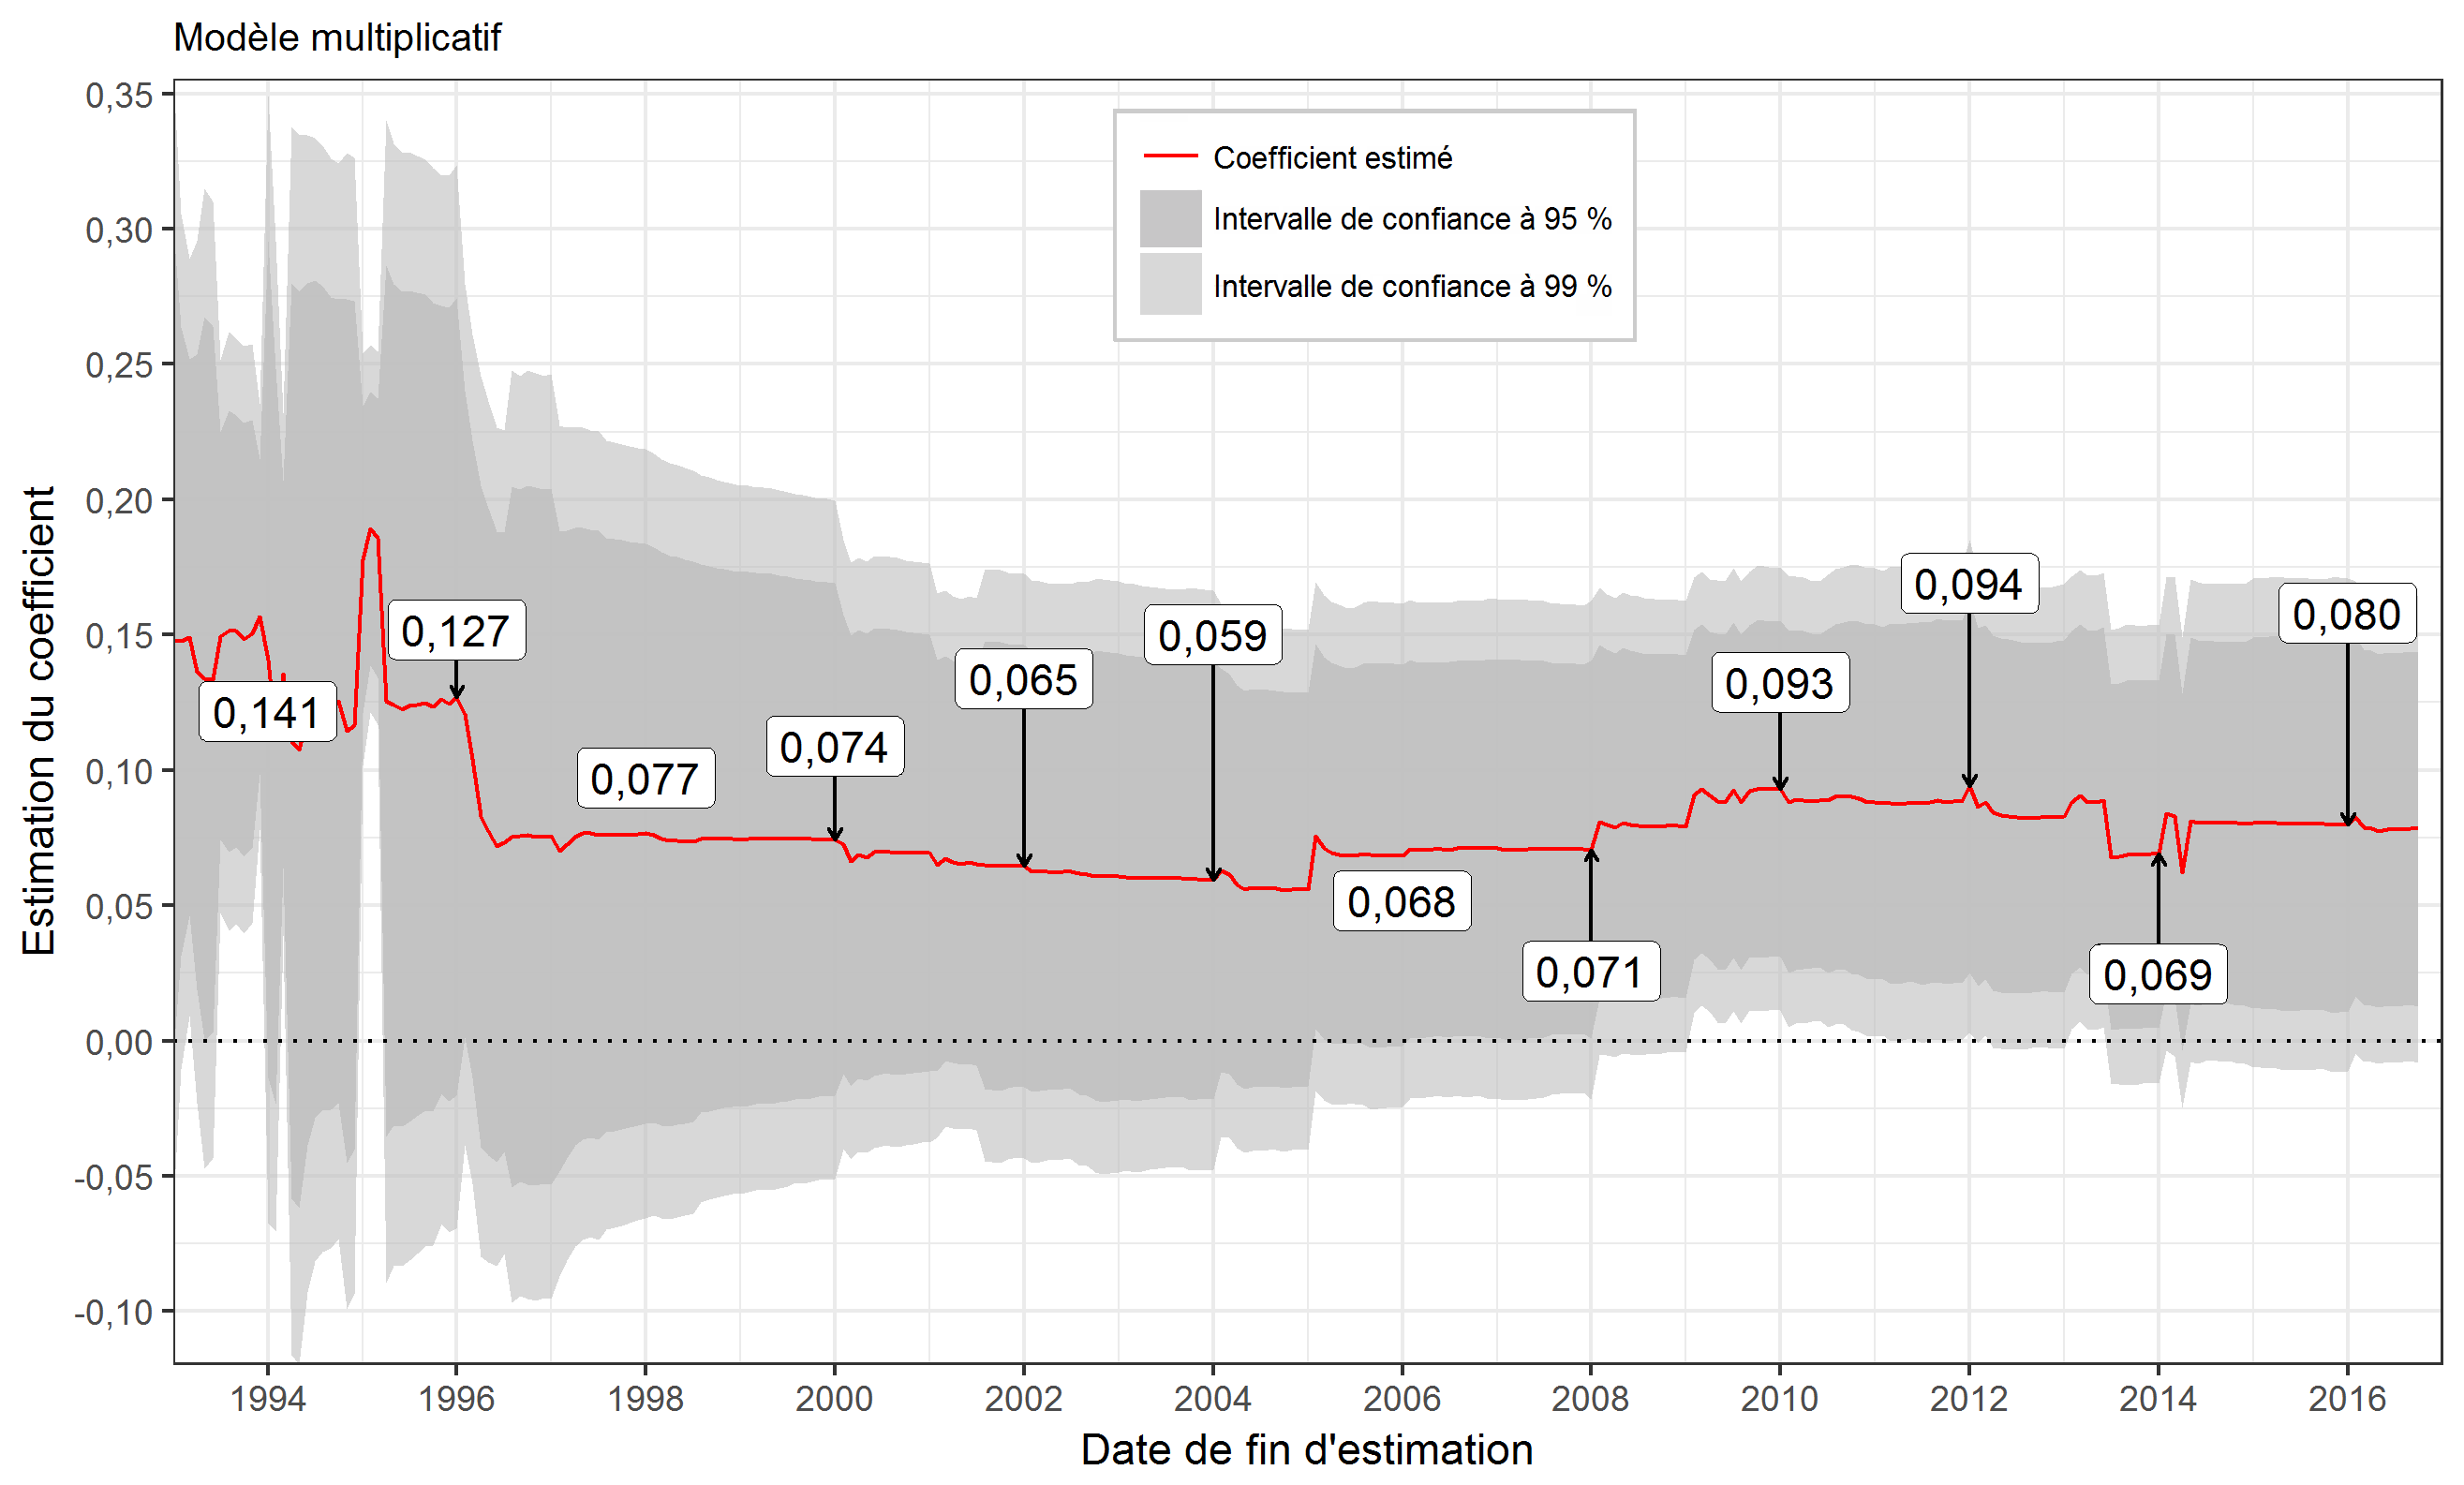
\includegraphics[scale=0.50]{img/LYexemple2.png}
 \caption[Estimations successives du coefficient LY pour la série RF139]{Estimations successives du coefficient LY pour la série RF1391.}
 \label{fig:LYexemple2}
\end{center}
\end{figure}

Les indicateurs de convergence ayant été calculés in fine sur 624 séries. Les graphiques (\ref{fig:LYconvergence}) et (\ref{fig:LYvaleur}) résument les résultats de la simulation, sous forme de «~violons~» : les violons sont des variantes des boxplots. Les traits horizontaux sont les quartiles de la distribution dont la forme de la boîte donne l'allure. 

En matière de temps nécessaire pour obtenir une estimation stable, le graphique (\ref{fig:LYconvergence}) permet d'affirmer que :
\begin{itemize}
	\item[$\bullet$] Pour les trois-quarts des séries, il faut au minimum 10 ans pour que l'effet LY converge. C'est une simple question de bon sens : au-dessous de 3 observations, il est le plus souvent impossible de mesurer avec fiabilité un phénomène, ici la différence entre les mois de février d'années normales et bissextiles.
	\item[$\bullet$] La nature du modèle, additif ou multiplicatif, influence peu la durée de convergence.
	\item[$\bullet$] La convergence semble plus rapide pour les séries de chiffre d'affaires que pour les séries de production industrielle.
\end{itemize}

\begin{figure}[!ht]
\begin{center}
 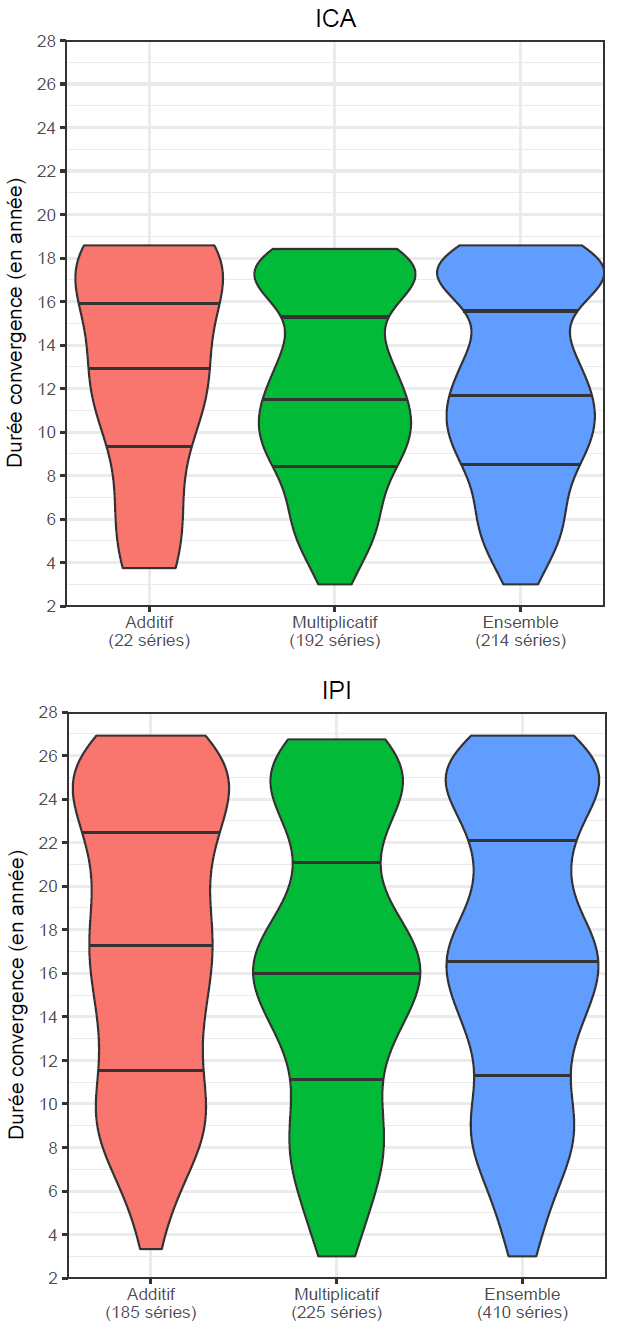
\includegraphics[scale=0.65]{img/LYconvergence2.png}
 \caption[Durée de convergence (en année) du coefficient LY (étude sur 624 séries)]{Durée de convergence (en année) du coefficient LY (étude sur 624 séries).}
 \label{fig:LYconvergence}
\end{center} \vspace{-0.3cm}
\footnotesize
\emph{Note de lecture : en ordonnée la densité de probabilité de la durée de convergence de l'estimation du régresseur année bissextile (LY). Les traits horizontaux représentent les quartiles associés (minimum, premier quartile, médiane, troisième quartile et maximum).}
\end{figure}

En ce qui concerne la valeur du coefficient, le graphique (\ref{fig:LYvaleur}) permet d'affirmer que :
\begin{itemize}
	\item[$\bullet$] Pour les modèles multiplicatifs, les indices de chiffre d'affaires (ICA) convergent vers une valeur médiane proche de la valeur attendue ($3,5~\%$) comme le souligne \cite{B1992}. Par contre, pour l'IPI, cette valeur médiane est plus forte, de l'ordre de 0,45 point.
	\item[$\bullet$] Pour les modèles additifs, les séries ICA convergent en médiane vers 3 points d'indice, ce qui correspond à peu près à la valeur attendue puisque les indices ne sont pas en général très différents de 100. Par contre, pour l'IPI, cette valeur médiane est plus forte, de l'ordre de 4,5 points.
	\item[$\bullet$] Pour de nombreuses séries, environ 20~\%, la valeur obtenue semble excessive : au delà de 6 points et parfois beaucoup plus.
\end{itemize}

\begin{figure}[!ht]
\begin{center}
 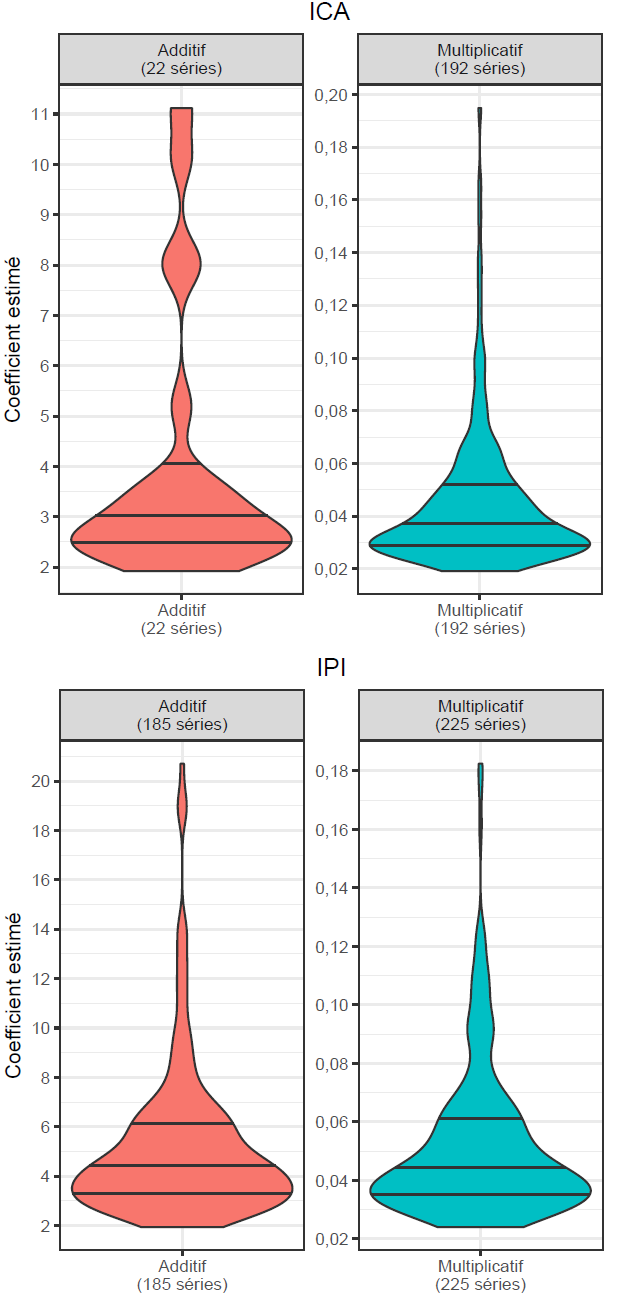
\includegraphics[scale=0.65]{img/LYvaleur2.png}
 \caption[Estimation finale de l'effet LY (étude sur 624 séries)]{Estimation finale de l'effet LY (étude sur 624 séries).}
 \label{fig:LYvaleur}
\end{center}
\vspace{-0.3cm}
\footnotesize\emph{Note de lecture : en ordonnée la densité de probabilité du coefficient de régression estimé du régresseur année bissextile (LY). Les traits horizontaux représentent les quartiles associés (minimum, premier quartile, médiane, troisième quartile et maximum).}
\end{figure}

\clearpage

En conclusion de cette première expérience, il semble illusoire de vouloir estimer sérieusement un effet «~année bissextile~» avec des séries qui en contiennent moins de 4, c'est à dire dans le meilleur des cas de moins de 13 ans.

De plus, se pose sérieusement la question de savoir s'il n'est pas préférable de corriger \emph{a priori} cet effet en l'estimant égal à 3,5~\%. Pour apporter des éléments de réponse à cette question, nous avons analysé l'ensemble des 2198 séries de deux façons :
\begin{enumerate}
	\item Modèle 1 : en corrigeant préalablement à la modélisation Reg-ARIMA la série brute par un coefficient correctif égal à :
$
\alpha_{t} = \left\{ \begin{array}{rl} 
                \frac{28,25}{29} & \mbox{si } t \mbox{ est un mois de février bissextil } \\
                \frac{28,25}{28} & \mbox{si } t \mbox{ est un mois de février non bissextil } \\
                1 & \mbox{sinon}
               \end{array}
         \right.
$
  \item Modèle 2 : en laissant le modèle Reg-ARIMA estimer l'effet «~année bissextile~» à partir du régresseur : $
LY_{t} = \left\{ \begin{array}{rl} 
                0,75 & \mbox{si } t \mbox{ est un mois de février bissextil } \\
                -0,25 & \mbox{si } t \mbox{ est un mois de février non bissextil } \\
                0 & \mbox{sinon}
               \end{array}
         \right.
$
\end{enumerate}

La qualité globale des ajustements est jugée alors par le critère d'Akaïké corrigé ($AICC$) : le modèle 1 est alors jugé meilleur que le modèle 2 si $(AICC1 \le AICC2)$. Les ajustements sont faits, comme précédemment, en rajoutant une observation à la fois.
Le graphique (\ref{fig:LYvaleur}) montre l'évolution du pourcentage de séries pour lesquelles $(AICC1 \le AICC2)$, en fonction du temps et du mode de décomposition.

Les résultats de cette expérience sont sans équivoque : 
\begin{itemize}
	\item [$\bullet$] Pour les modes de décomposition additifs, la correction manuelle est meilleure dans environ 85~\% des cas.
	\item [$\bullet$] Pour les modes de décomposition multiplicatifs, la correction manuelle est meilleure dans environ 80~\% des cas lorsque la série est suffisamment longue. Le pourcentage descend à 70-75~\% pour les séries plus courtes.
\end{itemize}

\begin{figure}[!ht]
\begin{center}
 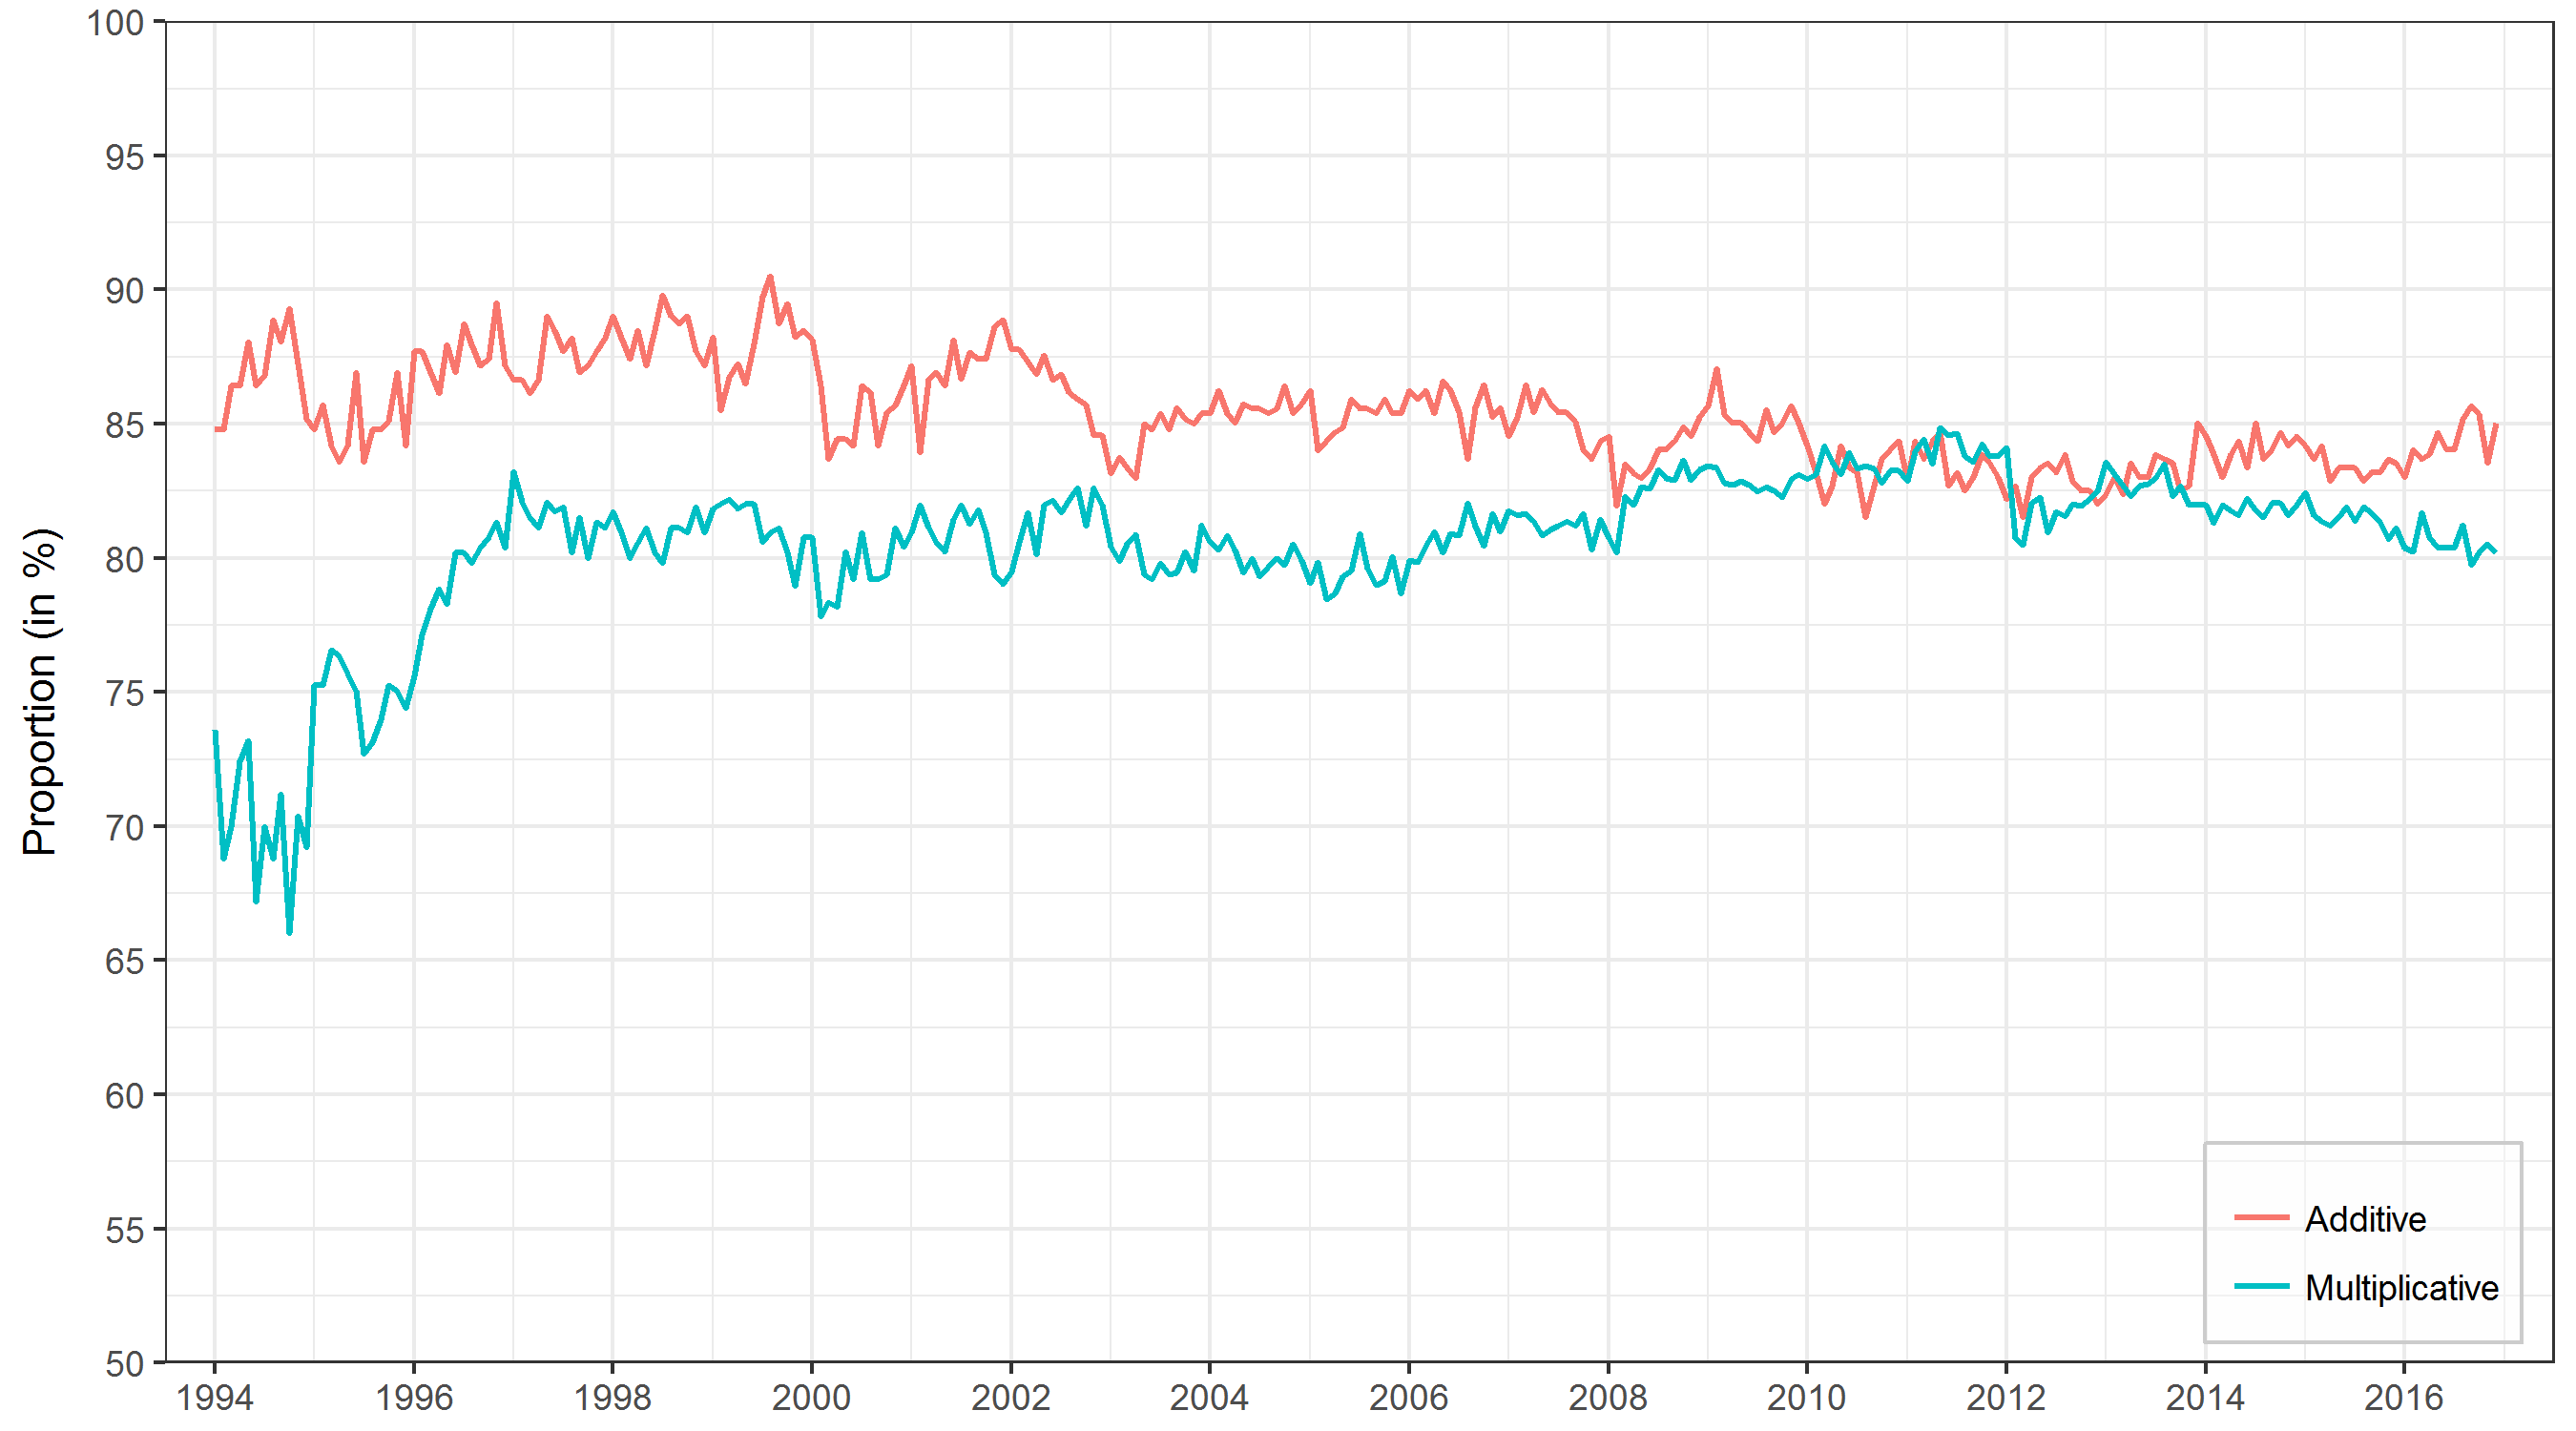
\includegraphics[scale=0.65]{img/LYaicc.png}
 \caption[Évolution du pourcentage de cas où le pré-ajustement manuel de l'effet «~année bissextile~» est meilleur (au sens du $AICC$) que le pré-ajustement Reg-ARIMA (étude sur 2198 séries)]{Évolution du pourcentage de cas où le pré-ajustement manuel de l'effet «~année bissextile~» est meilleur (au sens du $AICC$) que le pré-ajustement Reg-ARIMA (étude sur 2198 séries).}
 \label{fig:LYaicc}
\end{center}
\end{figure}

\clearpage

\section{Estimation de ruptures}
\label{sec:AO}

Dans cette partie, nous nous consacrons à l'estimation des points atypiques et ruptures définis au paragraphe \ref{sec:PAR}, et plus précisément les AO, LS, TC et SO.

\subsection{Méthodologie}

Nous utilisons les indices mensuels en volume de la production industrielle des pays de la communauté européenne, au niveau quatre chiffres de la NACE rev 2. Nous ne conservons, pour étudier la convergence des estimations, que les 12 premières années des séries.
La méthodologie retenue est très similaire à celle suivie dans la partie précédente. Cependant, pour comparer les résultats plus aisément, les séries sont corrigées des points atypiques l'année de l'introduction de la rupture et elles sont toutes rebasées à 100 le mois de l'introduction de la rupture.
\begin{enumerate}
	\item Le modèle de décomposition, les points atypiques, les ruptures, les effets de jours ouvrables et le modèle ARIMA sont identifiés et estimés sur l'ensemble de la série (12 ans). Le modèle Reg-ARIMA est donc déterminé.
	\item La série brute est corrigée des points atypiques l'année de l'introduction de la rupture et elle est rebasée à 100 au mois d'introduction de la rupture ($49^{\mbox{\tiny ème}}$ observation). Ces opérations ne modifient pas le modèle Reg-ARIMA\footnote{En revanche, dans le cas d'un schéma additif, le rebasement implique une modification des coefficients estimés qui sont multipliés par le coefficient de rebasement.}.
	\item Nous simulons une rupture à la $49^{\mbox{\tiny ème}}$ observation de la série, en rajoutant 10 fois le régresseur à la série si le modèle est additif, ou bien 1,1 fois le régresseur à la série si le modèle est multiplicatif.
	\item Le régresseur lié à la rupture étudiée est ajouté au modèle Reg-ARIMA et son coefficient est estimé sur les 49 premières observations de la série en figeant tous les autres paramètres estimés dans la première étape.
	\item Enfin, le processus est répété en ajoutant à chaque fois une observation, ce qui donne de nouvelles estimations des paramètres. Pour une série de 12 ans, nous aurons donc $12\times12 - 48 = 96$ estimations du coefficient du régresseur modélisant la rupture.
\end{enumerate}
Ces simulations permettent alors d'étudier la convergence du coefficient de la rupture. Dans cette étude, nous dirons que l'estimation du coefficient de la rupture aura convergé lorsqu'elle restera à moins de 5~\% en valeur absolue de la dernière estimation.

\subsection{Résultats}

\begin{figure}[!hb]
\begin{center}
 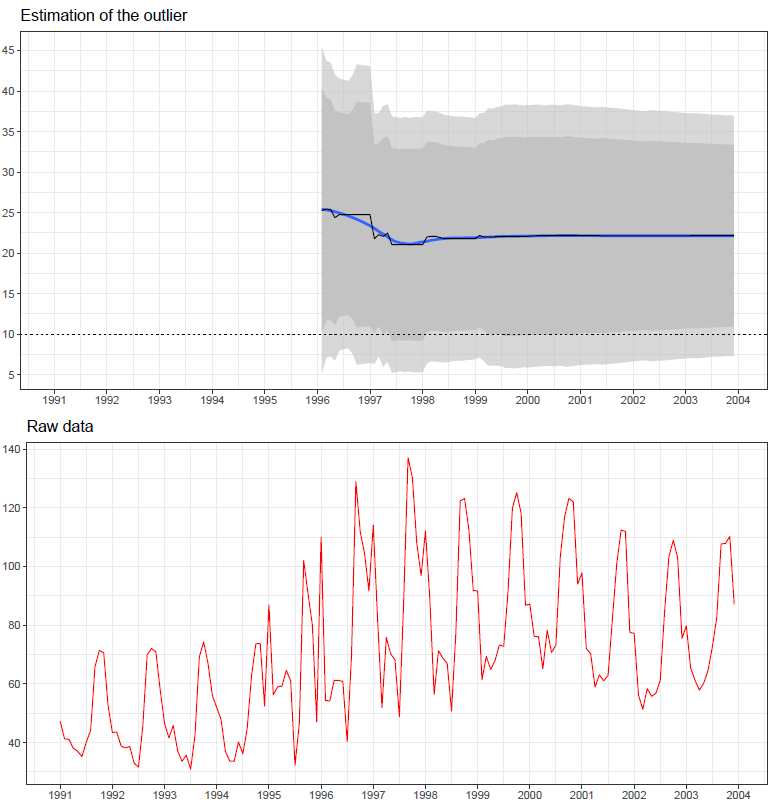
\includegraphics[width=16cm]{img/DE-C1062-EstimateAO.PNG}
 \caption[Série brute et évolution de l'estimation du point atypique AO1996.jan pour la série DE-C1062 (modèle additif)]{Série brute et évolution de l'estimation du point atypique AO1996.jan pour la série DE-C1062 (modèle additif).}
 \label{fig:DE-C1062}
\end{center}
\end{figure}

\begin{figure}[!ht]
\begin{center}
 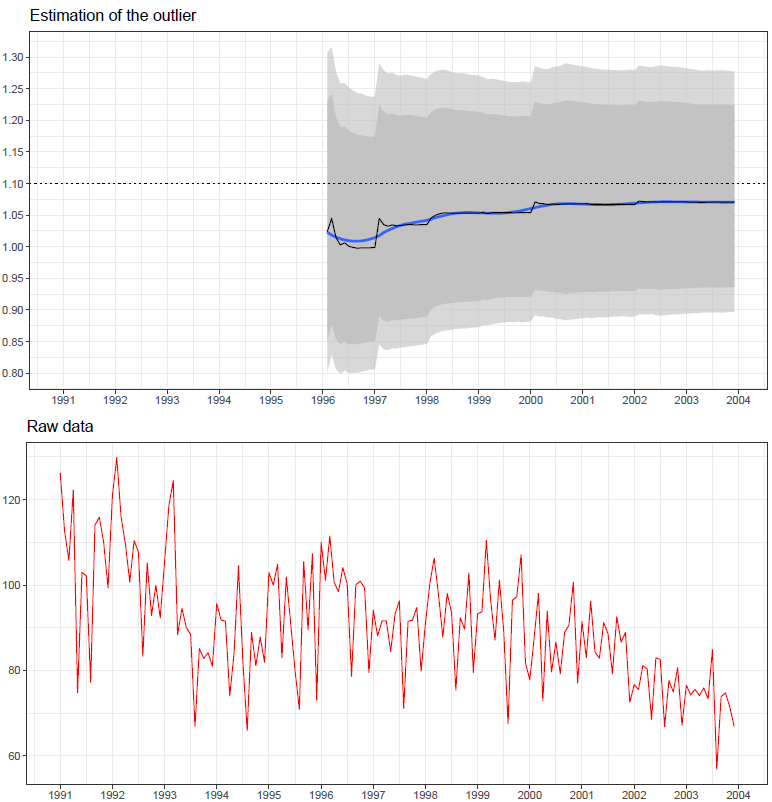
\includegraphics[width=16cm]{img/DE-C1086-EstimateAO.PNG}
 \caption[Série brute et évolution de l'estimation du point atypique AO1996.jan pour la série DE-C1086 (modèle multiplicatif)]{Série brute et évolution de l'estimation du point atypique AO1996.jan pour la série DE-C1086 (modèle multiplicatif).}
 \label{fig:DE-C1086}
\end{center}
\end{figure}

Les résultats sont représentés aux graphiques (\ref{fig:DE-C1062}) et (\ref{fig:DE-C1086}) ; dans ces graphiques, la courbe rouge est celle des estimations, la courbe bleue en est une version lissée, les zones grisées représentent les intervalles de confiance à 95~\% et 99~\%, et la ligne pointillée la vraie valeur de la rupture.
\begin{itemize}
	\item[$\bullet$] Dans les deux cas, on voit que le coefficient AO met du temps à converger et les valeurs des premières années peuvent être assez erratiques.
	\item[$\bullet$] La valeur même de l'estimation peut être très différente de la vraie valeur.
\end{itemize}

\vspace{2mm}

Les graphiques (\ref{fig:OutliersConvergence}) et (\ref{fig:OutliersValue}), ainsi que les tableaux (\ref{table:AOconvergence}) et (\ref{table:AOvaleur}) associés, résument les distributions de la durée de convergence et de la valeur estimée, pour 461 séries et les 4 types de ruptures étudiés :
\begin{itemize}
	\item[$\bullet$] En général, les estimations mettent beaucoup de temps à converger.
		\item[$\bullet$] Pour les modèles additifs 75~\% des séries, $SO$, $LS$ et $TC$ mettent environ 7 ans à converger, 5 ans pour les $AO$. En médiane, $AO$ et $TC$ mettent 4 ans à converger et les $LS$ et $SO$ 5 ans.
	\item[$\bullet$] La convergence semble encore moins rapide pour les modèles multiplicatifs puisque pour 75~\% des séries, les $AO$ mettent environ 6 ans à converger et les $SO$, $LS$ et $TC$ environ 7 ans. En revanche, en médiane, les $AO$, $LS$, $TC$ et $SO$ convergent en 4 ans.
	\item[$\bullet$] En médiane, les estimations des diverses ruptures convergent à peu près vers la valeur attendue. Mais dans 50~\% des cas la valeur estimée converge à environ $\pm$ 30~\% de la vraie valeur. On peut noter aussi la présence d'estimations aberrantes dont certaines traduisent même des baisses au lieu de la hausse modélisée.

\end{itemize}

\begin{figure}[h!]
\begin{center}
 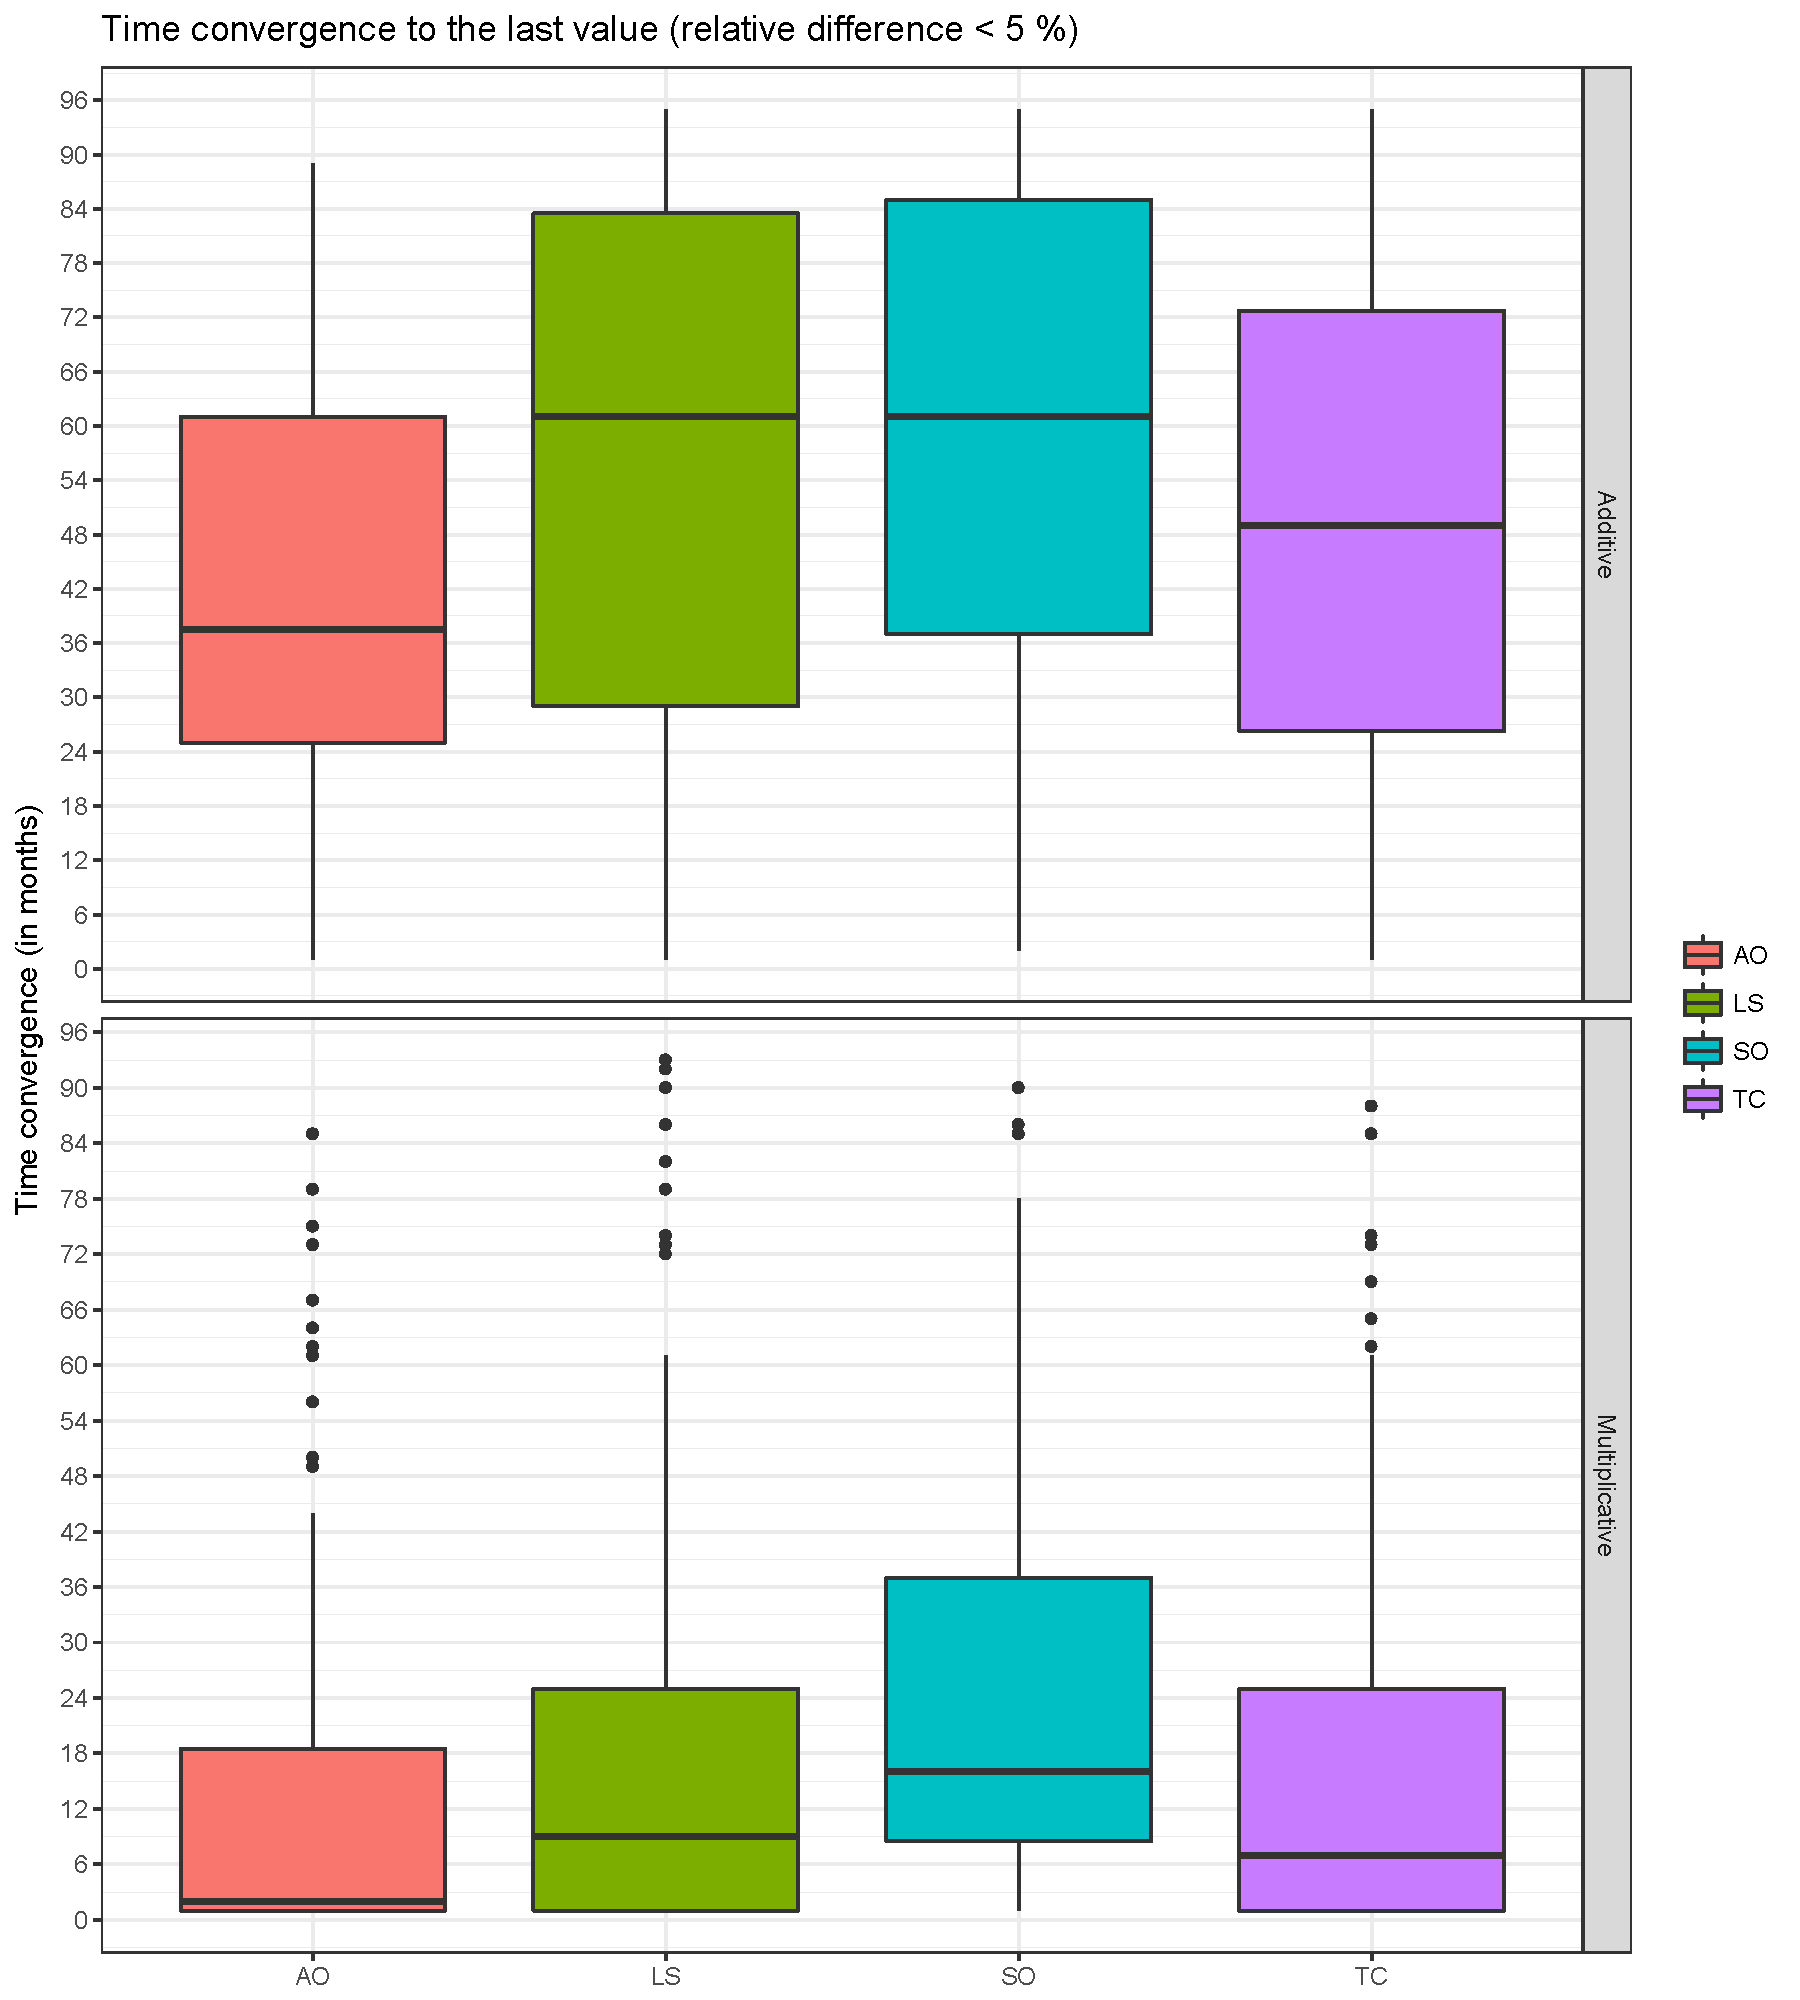
\includegraphics[scale=0.65]{img/OutliersConvergence.png}
 \caption[Durée de convergence (en mois) du coefficient de la rupture selon le modèle de décomposition]{Durée de convergence (en mois) du coefficient de la rupture selon le modèle de décomposition.}
 \label{fig:OutliersConvergence}
\end{center}
\end{figure}

\begin{figure}[!ht]
\begin{center}
 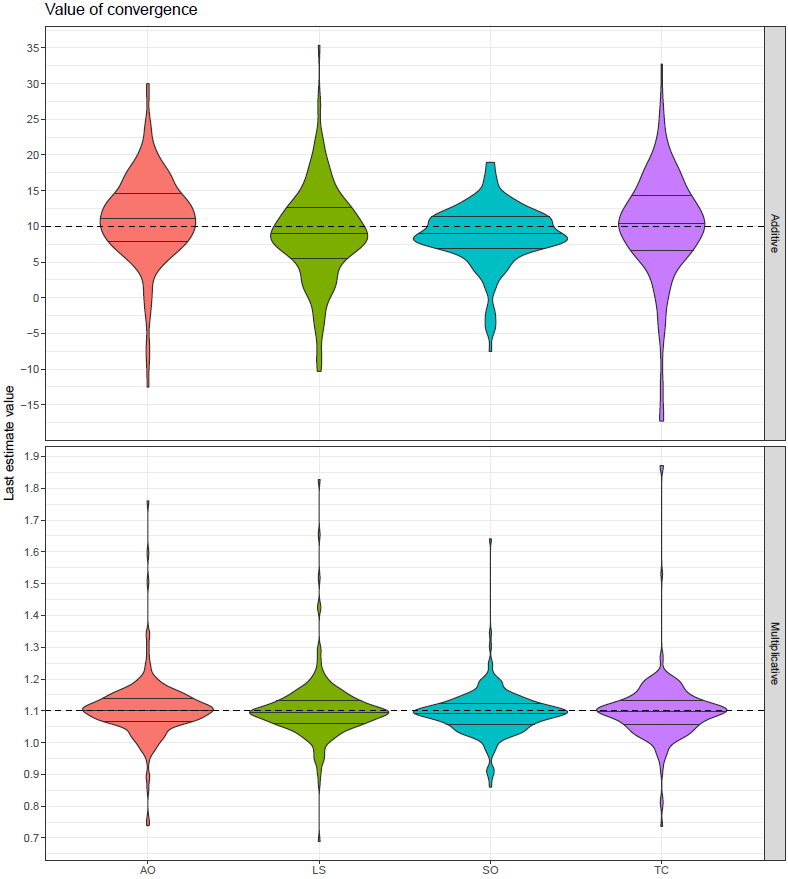
\includegraphics[scale=0.65]{img/OutliersValue.png}
 \caption[Estimation finale du coefficient de la rupture selon le modèle de décomposition]{Estimation finale du coefficient de la rupture selon le modèle de décomposition.}
 \label{fig:OutliersValue}
\end{center}\vspace{-0.3cm}
\footnotesize
\emph{Note de lecture : en ordonnée la densité de probabilité du coefficient de régression estimé de la rupture étudiée. Les traits horizontaux représentent les quartiles associés (minimum, premier quartile, médiane, troisième quartile et maximum).}
\end{figure}

\clearpage

\begin{table}[h]
\caption[Statistiques sur la durée de convergence (en mois) du coefficient de la rupture selon le modèle de composition et le type de rupture]{Statistiques sur la durée de convergence (en mois) du coefficient de la rupture selon le modèle de composition et le type de rupture.} \label{table:AOconvergence}
\begin{center}
\begin{tabular}{lccccc}
\toprule
  & Minimum & 25 \% & 50 \% & 75 \% & Maximum\\
\midrule
\addlinespace[0.3em]
\multicolumn{6}{l}{\textbf{Modèles additifs}}\\
\hspace{1em}AO & 1 & 25 & 42 & 62 & 91\\
\hspace{1em}LS & 1 & 31 & 61 & 84 & 95\\
\hspace{1em}SO & 2 & 37 & 61 & 75 & 90\\
\hspace{1em}TC & 1 & 26 & 49 & 73 & 94\\
\addlinespace[0.3em]
\multicolumn{6}{l}{\textbf{Modèles multiplicatifs}}\\
\hspace{1em}AO & 1 & 14 & 49 & 74 & 95\\
\hspace{1em}LS & 1 & 24 & 50 & 85 & 95\\
\hspace{1em}SO & 1 & 25 & 50 & 85 & 95\\
\hspace{1em}TC & 1 & 17 & 54 & 84 & 95\\
\bottomrule
\end{tabular}
\end{center}
\end{table}

\begin{table}[h]
\caption[Statistiques sur les valeurs de convergence selon le modèle de composition et le type de rupture. Les valeurs attendues sont +10 pour les modèles additifs et 1,10 (+10~\%) pour les modèles multiplicatifs]{Statistiques sur les valeurs de convergence selon le modèle de composition et le type de rupture. Les valeurs attendues sont +10 pour les modèles additifs et 1,10 (+10~\%) pour les modèles multiplicatifs.}\label{table:AOvaleur} 
\begin{center}
\begin{tabular}{lccccc}
\toprule
  & Minimum & 25 \% & 50 \% & 75 \% & Maximum\\
\midrule
\addlinespace[0.3em]
\multicolumn{6}{l}{\textbf{Modèles additifs}}\\
\hspace{1em}AO & -11,6 & 7,8 & 11,1 & 14,2 & 36,9\\
\hspace{1em}LS & -11,4 & 5,6 & 9,3 & 12,7 & 49,8\\
\hspace{1em}SO & -5,8 & 7,3 & 8,8 & 11,0 & 31,1\\
\hspace{1em}TC & -17,4 & 6,5 & 10,2 & 14,1 & 47,2\\
\addlinespace[0.3em]
\multicolumn{6}{l}{\textbf{Modèles multiplicatifs}}\\
\hspace{1em}AO & 0,72 & 1,07 & 1,10 & 1,14 & 1,88\\
\hspace{1em}LS & 0,68 & 1,07 & 1,10 & 1,13 & 1,81\\
\hspace{1em}SO & 0,86 & 1,06 & 1,10 & 1,12 & 1,40\\
\hspace{1em}TC & 0,73 & 1,06 & 1,10 & 1,14 & 1,87\\
\bottomrule
\end{tabular}
\end{center}
\end{table}


\clearpage

\section{L'estimation du modèle ARIMA}

Nous arrivons maintenant dans la partie certainement la plus dérangeante de cette étude. Dans l'exemple proposé, la série suit un modèle additif et le modèle Reg-ARIMA général s'écrit :
\begin{eqnarray}
	\label{eq:eq4}
z_t=\beta_0 LY_t + \sum_{j=1}^{j=6} \beta_j \left(N_{jt} - N_{7t}\right) + \sum_{l=1}^{l=k} \alpha_l O_{lt} + x_t,
\end{eqnarray}
où les $O_l$ ($l=1, \cdots, k$) désignent les ruptures qui seront éventuellement détectées par l'algorithme. Dans cette formulation on peut :
\begin{enumerate}
	\item Soit laisser le régresseur LY dans le système de régresseurs pour jours ouvrables généré automatiquement par l'algorithme ;
	\item Soit enlever LY de ce système et l'introduire comme régresseur externe.
\end{enumerate}
Les deux modèles sont parfaitement équivalents du point de vue théorique. Mais les algorithmes, mise en œuvre de la théorie, ne sont pas la théorie ! Et de fait, les estimations du même modèle dans des conditions légèrement différentes peuvent générer des résultats sensiblement différents. Ainsi, si on fait l'expérience sur la série RF241 de l'IPI français, on obtient (voir figure \ref{fig:CholeskyRF241}) :
\begin{itemize}
	\item[$\bullet$] Dans le cas où LY est généré dans les régresseurs pour jours ouvrables : un effet LY significatif (au seuil de 5~\%), les effets de calendrier (jours ouvrables et effet LY) sont significatifs (au seuil de 5~\%), 3 ruptures et un modèle ARIMA $(2,0,0)(0,1,1)$ ;
	\item[$\bullet$] Et dans le cas où LY est considéré comme régresseur externe : un effet LY significatif (au seuil de 5~\%), pas d'effet jours ouvrables, 8 ruptures et un modèle ARIMA $(0,1,1)(0,1,1)$ ;
%	\item[$\bullet$] Il se trouve que le modèle obtenu avec LY en régresseur externe, est sensiblement meilleur du point de vue du critère d'Akaïké corrigé.
\end{itemize}

Heureusement ce phénomène surprenant est relativement rare. Il tient au fait que dans le second cas le modèle est mal spécifié : en n'introduisant pas le régresseur LY dans les effets de calendrier, ils sont considérés comme significativement nuls et ne sont donc pas retenus par l'algorithme. Il en découle ensuite un différent modèle ARIMA et des différentes ruptures.
%Il tient l'algorithme utilise des factorisations de Cholesky pour calculer des inverses et des déterminants de matrices et que ces factorisations ne sont pas toujours uniques. Dans ce cas, l'ordre dans lequel les variables interviennent dans la matrice peut conduire à des décompositions différentes et in fine à des résultats différents.

\begin{figure}[!ht]
\begin{center}
 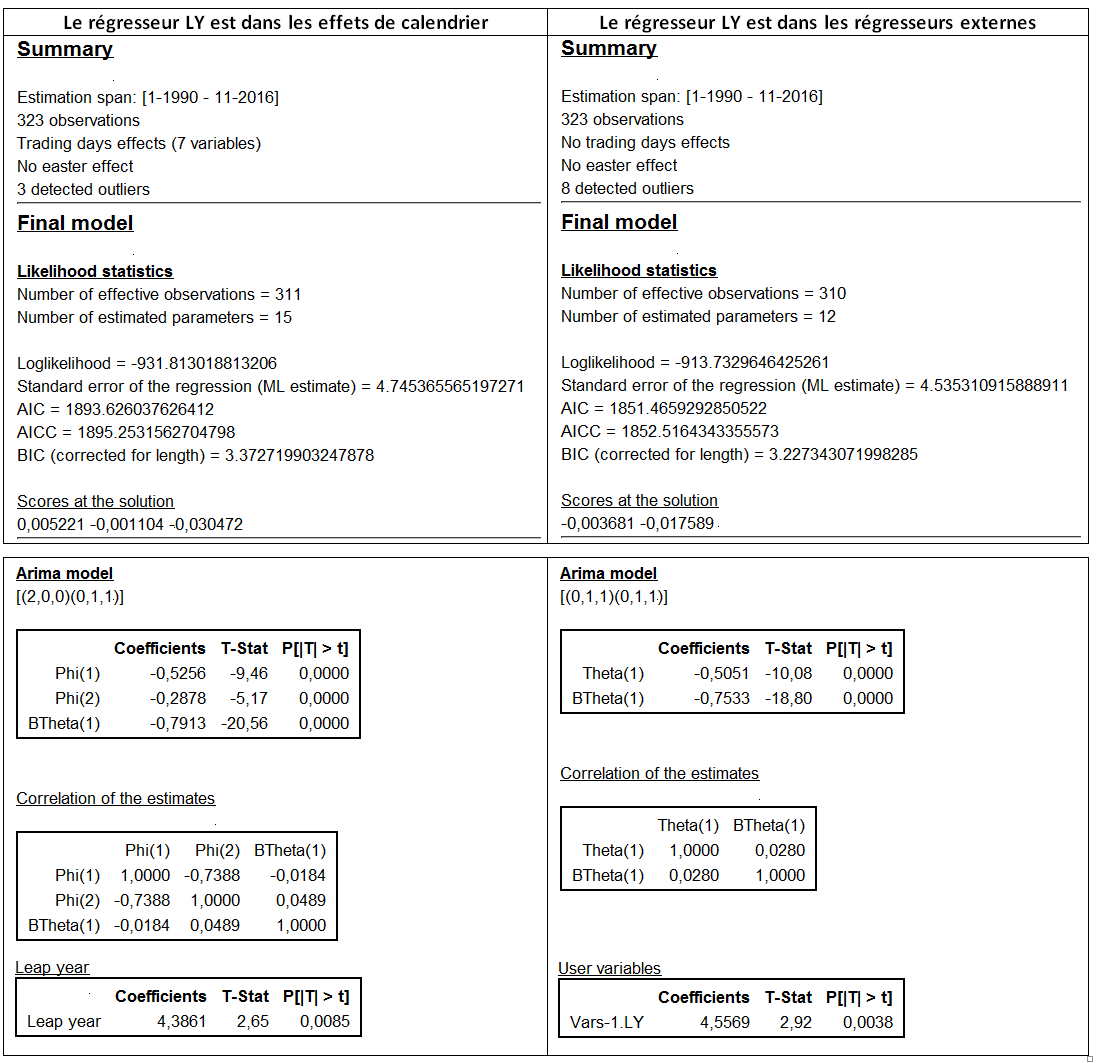
\includegraphics[width=16cm]{img/CholeskyRF241.png}
 \caption[Comparaison des modèles obtenus pour la série RF241 selon que le régresseur LY est mis en régresseur externe ou non]{Comparaison des modèles obtenus pour la série RF241 selon que le régresseur LY est mis en régresseur externe ou non.}
 \label{fig:CholeskyRF241}
\end{center}
\end{figure}


\clearpage

\section*{Conclusion \markboth{Conclusion}{Conclusion}}
\addcontentsline{toc}{section}{Conclusion}

Les modèles Reg-ARIMA sont des modèles paramétriques qui, comme de nombreuses méthodes paramétriques, sont très sensibles aux valeurs atypiques et au respect des hypothèses sur lesquels ils reposent. Ce manque de robustesse est connu depuis des décennies et est à l'origine de la statistique robuste\footnote{Voir par exemple \cite{T1977} et \cite{HR2011}.}.

Pour bien les utiliser, il est essentiel de bien spécifier \textbf{au préalable} le modèle et de vérifier que les hypothèses du modèle sont bien remplies. Ainsi :
\begin{itemize}
  \item[$\bullet$] même si les utilisateurs sont friands de séries longues, il est extrêmement peu probable qu'une série économique suivent le même modèle ARIMA sur plus de 15 ans. En particulier, les rebasements et changements de nomenclature amènent souvent à rétropoler les séries avec des indicateurs proches mais à dynamique sans doute différente. Une série longue doit donc être désaisonnalisée par sous périodes --- voir à cet égard \cite{E2015} et \cite{PQLT2018} ;
	\item[$\bullet$] un effet de Pâques sur les séries de la production industrielle est très peu probable, sauf peut-être pour quelques niveaux très fins de la nomenclature ;
	\item[$\bullet$] le système de régresseurs pour jours ouvrables doit être basé sur des considérations économiques plus que statistiques (voir l'exemple sur l'effet «~année bissextile~»). À cet égard, il est intéressant de noter que les systèmes proposés par défaut par les méthodes actuelles (6 régresseurs, un pour chaque jour de la semaine, ou 1 régresseur représentant les 5 jours de la semaine hors weekend) sont soit instables, soit inadéquats comme le montrent \cite{A2012} ou \cite{L2018}.
\end{itemize}

\vskip \baselineskip
En matière de désaisonnalisation, la plupart des instabilités évoquées n'auront qu'un effet limité sur la série désaisonnalisée et corrigée des effets de jours ouvrables\footnote{En particulier parce que les ruptures AO, LS et TC sont réintroduites dans la séries désaisonnalisée en fin de traitement et parce que les effets de calendrier sont en général faibles.}, surtout si \textsc{X-13Arima-Seats} est utilisé. Mais elles changeront sans aucun doute l'histoire à court-terme et introduiront éventuellement des révisions désagréables.

\vskip \baselineskip
Les simulations présentées dans cet exercice sont certainement critiquables et améliorables mais elles ont le mérite de mettre le doigt sur la potentielle instabilité de ces modèles Reg-ARIMA souvent utilisés comme des boîtes noires. Les algorithmes automatiques mis en œuvre dans les méthodes \textsc{X-13Arima-Seats} et \textsc{Tramo-Seats} sont cependant des outils importants et très utiles. Le mieux est certainement de les utiliser en respectant les principes des «~lignes directrices européennes pour la désaisonnalisation~» publiées par \cite{E2015}.

Baser par exemple des procédures de choix de systèmes de régresseurs pour jours ouvrables ou plus généralement de paramètres de désaisonnalisation sur ces modèles, sans s'appuyer sur un raisonnement économique et la connaissance du domaine étudié, serait une grosse erreur\dots qui amènerait sans doute à dire de vous : «~\textit{Il se sert des statistiques comme un ivrogne d'un réverbère : pour se soutenir et non pour s'éclairer.}~»\footnote{\textit{«~He uses statistics as a drunken man uses lamp posts, for support rather than illumination~»}. Citation largement attribuée à Andrew Lang (1844-1912), écrivain écossais, mais la citation originale n'a jamais été retrouvée.}

\newpage
\appendix
\section{Le calendrier grégorien}
\label{sec:cal}

Le calendrier grégorien est un calendrier solaire, basé sur le mouvement de la Terre autour du Soleil, et pour lequel l'année est une approximation de l'année tropicale, durée que la Terre prend pour aller d'un point fixe, comme un équinoxe ou un solstice, au suivant. Dans ce calendrier, une année normale est faite de 12 mois --- janvier, février, mars, avril, mai, juin, juillet, août, septembre, octobre, novembre et décembre --- qui contiennent un nombre de jours égal respectivement à 31, 28, 31, 30, 31, 30, 31, 31, 30, 31, 30 et 31. Une année normale contient donc 365 jours, ce qui est malheureusement un peu trop court dans la mesure où la Terre met environ 365 jours et 6 heures pour accomplir une révolution autour du soleil. Une meilleure approximation de l'année solaire est obtenue en ajoutant 1 jour à certaines années, les années bissextiles, pour lesquelles le mois de février aura 29 jours. Une année bissextile est une année divisible par 4 mais pas par 100, sauf si elle est divisible par 400. Ainsi, 1900 ne fut pas une année bissextile, 2000 en était une et 2100 ne sera pas bissextile. On a donc \emph{in fine} 97 années bissextiles sur une période de 400 ans. Il reste cependant une petite erreur d'approximation d'environ 1 jour tous les 4000 ans que le calendrier grégorien ne prend pas en compte.

Toute période de 400 ans contient donc $400 \times 365 + 97 = 146097$ jours, soit exactement $20871$ semaines. Le calendrier grégorien est donc périodique de période 400 ans. La longueur moyenne d'une année sur ce cycle est de $146097 / 400 = 365,2425$ jours et la longueur moyenne d'un mois est de $365,2425 / 12 = 30,436875$ jours.

\newpage
 
\nocite{*}
\begin{thebibliography}{999}
\bibitem[Attal-Toubert (2012)]{A2012} Attal-Toubert, K. (2012), Régresseurs pour effets de calendrier : comment les construire, comment les choisir ? Actes des $11^{\mbox{\tiny èmes}}$ Journées de Méthodologie Statistique, \url{http://jms-insee.fr/jms2012s14_3/}.
\bibitem[Bell (1992)]{B1992} Bell, W. R. (1992), Alternative Approaches to Length of Month Adjustment, Research Report Series 1992-17, Satistical Research Division, U. S. Census Bureau, Washington DC. \url{https://www.census.gov/ts/papers/rr92-17.pdf}.
\bibitem[Eurostat (2015)]{E2015} Eurostat (2015), The ESS guidelines for seasonal adjustment, Eurostat manuals and guidelines, Product Code: KS-GQ-15-001. \url{http://ec.europa.eu/eurostat/web/products-manuals-and-guidelines/-/KS-GQ-15-001}.
\bibitem[Findley et McElroy (2018)]{FMcE2018} Findley, D., McElroy, T. (2018), Background and Perspectives for ARIMA Model-Based Seasonal Adjustment, in Handbook on Seasonal Adjustment, edited by G. L. Mazzi, co-edited by D. Ladiray, European Union, Luxembourg. \url{ec.europa.eu/eurostat/web/products-manuals-and-guidelines/-/KS-GQ-18-001}.
\bibitem[Findley et al. (1998)]{FMBOC1998} Findley, D.F., Monsell, B.C., Bell, W.R., Otto, M.C., Chen, B.C. (1998), New capabilities and methods of the X-12-ARIMA seasonal adjustment program, Journal of Business and Economic Statistics, 16, 127-152.
\bibitem[G\'{o}mez et Maravall (1996)]{GM1996} G\'{o}mez, V. and Maravall, A. (1996), Programs TRAMO and SEATS. Instructions for the User, (with some updates), Working Paper 9628, Servicio de Estudios, Banco de Espa\~{n}a.
\bibitem[G\'{o}mez et Maravall (1998)]{GM1998} G\'{o}mez, V., Maravall, A. (1998), Automatic Modeling Methods For Univariate Series, Working Paper 9808, Servicio de Estudios, Banco de Espa\~{n}a.
\bibitem[Grudkowska (2017)]{G2017} 	Grudkowska, S. (2017),	JDemetra+ Reference Manual Version 2.2, available from URL: \url{https://ec.europa.eu/eurostat/cros/content/software-jdemetra_en}.
\bibitem[Huber et Ronchetti (2011)]{HR2011} Huber, P. J., Ronchetti, E. M. (2011), Robust Statistics, Wiley Series in Probability and Statistics, John Wiley and Sons.
\bibitem[Ladiray et Quenneville (2001)]{LQ2001} Ladiray, D., Quenneville, B. (2001), Seasonal Adjustment with the X-11 Method, Lecture Notes in Statistics No 158, Springer, New York. Disponible en français sur \url{https://www.census.gov/ts/papers/x11_french.pdf}.
\bibitem[Ladiray (2018)]{L2018} Ladiray, D. (2018), Calendar effects, in Handbook on Seasonal Adjustment, edited by G. L. Mazzi, co-edited by D. Ladiray, European Union, Luxembourg. \url{ec.europa.eu/eurostat/web/products-manuals-and-guidelines/-/KS-GQ-18-001}.
\bibitem[Maravall et Caporello (2004)]{MC2004} Maravall, A., Caporello, G. (2004), Program TSW: Revised reference manual. Technical Report, Research Department, Bank of Spain.
\bibitem[Maravall et al. (2015)]{MLP2015} Maravall, A., L\'{o}pez, R., and P\'{e}rez, D. (2015), Reliability of the Automatic Identification of ARIMA Models in Program TRAMO, in Beran, J., Feng, Y., and Hebbel, H. (eds.) Empirical Economic and Financial Research. Theory, Methods and Practice, Springer International Publishing, Switzerland, 105-122.
\bibitem[Maravall et al. (2016)]{MLP2016} Maravall, A., L\'{o}pez, R., and P\'{e}rez, D. (2016), Reg-ARIMA Model Identification: Empirical Evidence, Statistica Sinica, 26, 1365-1388.
\bibitem[Maravall (2018)]{M2018} Maravall, A. (2018), Quality of Seasonal Adjustment in the Model-Based Approach of TRAMO-SEATS, in Handbook on Seasonal Adjustment, edited by G. L. Mazzi, co-edited by D. Ladiray, European Union, Luxembourg. \url{ec.europa.eu/eurostat/web/products-manuals-and-guidelines/-/KS-GQ-18-001}.
\bibitem[Mehrhoff (2018)]{Me2018} Mehrhoff, J. (2018), Outlier Detection and Correction, in Handbook on Seasonal Adjustment, edited by G. L. Mazzi, co-edited by D. Ladiray, European Union, Luxembourg. \url{ec.europa.eu/eurostat/web/products-manuals-and-guidelines/-/KS-GQ-18-001}.
\bibitem[Pham et Quartier-la-Tente (2018)]{PQLT2018} Pham, H., Quartier-la-Tente, A. (2018), Désaisonnaliser les séries très longues par sous-période, gains et choix de la longueur de traitement - exemple des séries de l'IPI, Actes des $13^{\mbox{\tiny èmes}}$ Journées de Méthodologie Statistique. 
\bibitem[Tukey (1977)]{T1977} Tukey, J. W. (1977), Exploratory Data Analysis, Addison-Wesley Publishing Company.





\end{thebibliography}

%\bibliography{DB}

\end{document}  